% !TeX spellcheck = en_US

%
% FH Technikum Wien
% !TEX encoding = UTF-8 Unicode
%
% Erstellung von Master- und Bachelorarbeiten an der FH Technikum Wien mit Hilfe von LaTeX und der Klasse TWBOOK
%
% Um ein eigenes Dokument zu erstellen, müssen Sie folgendes ergänzen:
% 1) Mit \documentclass[..] einstellen: Master- oder Bachelorarbeit, Studiengang und Sprache
% 2) Mit \newcommand{\FHTWCitationType}.. Zitierstandard festlegen (wird in der Regel vom Studiengang vorgegeben - bitte erfragen)
% 3) Deckblatt, Kurzfassung, etc. ausfüllen
% 4) und die Arbeit schreiben (die verwendeten Literaturquellen in Literatur.bib eintragen)
%
% Getestet mit TeXstudio mit Zeichenkodierung ISO-8859-1 (=ansinew/latin1) und MikTex unter Windows
% Zu beachten ist, dass die Kodierung der Datei mit der Kodierung des paketes inputenc zusammen passt!
% Die Kodierung der Datei twbook.cls MUSS ANSI betragen!
% Bei der Verwendung von UTF8 muss dnicht nur die Kodierung des Dokuments auf UTF8 gestellt sein, sondern auch die des BibTex-Files!
%
% Bugreports und Feedback bitte per E-Mail an latex@technikum-wien.at
%
% Versionen
% *) V0.7: 9.1.2015, RO: Modeline angepasst und verschoben
% *) V0.6: 10.10.2014, RO: Weitere Anpassung an die UK
% *) V0.5: 8.8.2014, WK: Literaturquellen überarbeitet und angepasst
% *) V0.4: 4.8.2014, WK: Initalversion in SVN eingespielt
%
\documentclass[MGS,Master,english]{twbook}%\documentclass[Bachelor,BMR,german]{twbook}
\usepackage[utf8]{inputenc}
\usepackage[T1]{fontenc}
\usepackage{graphicx}
%\usepackage[disable]{todonotes} % notes not showed
\usepackage[draft]{todonotes} % notes showed
\usepackage{verbatim} %multiline comment
\usepackage{longtable}
\usepackage{lscape}
\usepackage{nameref}

%
% Bitte in der folgenden Zeile den Zitierstandard festlegen
\newcommand{\FHTWCitationType}{HARVARD} % IEEE oder HARVARD möglich - wenn Sie zwischen IEEE und HARVARD wechseln, bitte die temorären Dateien (aux, bbl, ...) löschen
%
\ifthenelse{\equal{\FHTWCitationType}{HARVARD}}{\usepackage{harvard}}{\usepackage{bibgerm}}

% Definition Code-Listings Formatierung:
\usepackage[final]{listings}
\lstset{captionpos=b, numberbychapter=false,caption=\lstname,frame=single, numbers=left, stepnumber=1, numbersep=2pt, xleftmargin=15pt, framexleftmargin=15pt, numberstyle=\tiny, tabsize=3, columns=fixed, basicstyle={\fontfamily{pcr}\selectfont\footnotesize}, keywordstyle=\bfseries, commentstyle={\color[gray]{0.33}\itshape}, stringstyle=\color[gray]{0.25}, breaklines, breakatwhitespace, breakautoindent}
\lstloadlanguages{[ANSI]C, C++, [gnu]make, gnuplot, Matlab}

%Formatieren des Quellcodeverzeichnisses
\makeatletter
% Setzen der Bezeichnungen für das Quellcodeverzeichnis/Abkürzungsverzeichnis in Abhängigkeit von der eingestellten Sprache
\providecommand\listacroname{}
\@ifclasswith{twbook}{english}
{%
    \renewcommand\lstlistingname{Code}
    \renewcommand\lstlistlistingname{List of Code}
    \renewcommand\listacroname{List of Abbreviations}
}{%
    \renewcommand\lstlistingname{Quellcode}
    \renewcommand\lstlistlistingname{Quellcodeverzeichnis}
    \renewcommand\listacroname{Abkürzungsverzeichnis}
}
% Wenn die Option listof=entryprefix gewählt wurde, Definition des Entyprefixes für das Quellcodeverzeichnis. Definition des Macros listoflolentryname analog zu listoflofentryname und listoflotentryname der KOMA-Klasse
\@ifclasswith{scrbook}{listof=entryprefix}
{%
    \newcommand\listoflolentryname\lstlistingname{}
}{%
}
\makeatother
\newcommand{\listofcode}{\phantomsection\lstlistoflistings}

%
% Einträge für Deckblatt, Kurzfassung, etc.
%
\title{Using Procedural Content Generation via Machine Learning as a Game Mechanic}
\author{Bernhard Rieder, BSc}
\studentnumber{1610585006}
%\author{Titel Vorname Name, Titel\and{}Titel Vorname Name, Titel}
%\studentnumber{XXXXXXXXXXXXXXX\and{}XXXXXXXXXXXXXXX}
\supervisor{Dipl.-Ing. (FH) Alexander Hofmann}
%\supervisor[Begutachter]{Titel Vorname Name, Titel}
%\supervisor[Begutachterin]{Titel Vorname Name, Titel}
\secondsupervisor{Dr. Jichen Zhu \and{} Dr. Santiago Onta\~{n}\'{o}n}
%\secondsupervisor[Begutachter]{Titel Vorname Name, Titel}
%\secondsupervisor[Begutachterinnen]{Titel Vorname Name, Titel}
\place{Philadelphia}
\kurzfassung{{\color{blue}Blah blah blah, das ist meine Kurzfassung über die Verwendung von Prozeduraler Inhaltsgenerierung mit Machine Learning als eine Spielmechanik, blah blah blah}}
\schlagworte{{\color{blue}Prozedurale Inhaltsgenerierung, Machine Learning, Spielemechanik, Künstliche Intelligenz, Spieleentwicklung}}
\outline{
	{\color{blue}Blah blah blah, this is my outline about the use of procedural content generation via machine learning as a game mechanic, blah blah blah\\
	\\
	\textit{Procedural Content Generation (PCG) is an essential topic in modern games. Notably, it is a very crucial topic for independent game developers due to a low budget, where PCG can generate much content for less effort. As the importance of PCG for game development increases, researchers explore new avenues for generating high-quality content with or without human involvement. Here is where Machine Learning comes into play and extends the capabilities of PCG. Procedural Content	Generation via Machine Learning (PCGML) systems can be trained on its own and evolve if they do not generate usable output and offer a broad application possibility. One promising way of using PCGML is the use as a game mechanic. Therefore, this research will address and focus on the possibilities and development process of how PCGML can be used as a game mechanic and is going to provide a firrst demonstration of its use.}\\
	\\
	Abstracts can vary in length from one paragraph to several pages, but they follow the IMRaD format and
	typically spend:
	\begin{itemize}
		\item 25\% of their space on importance of research (Introduction)
		\item 25\% of their space on what you did (Methods)
		\item 35\% of their space on what you found: this is the most important part of the abstract (Results)
		\item 15\% of their space on the implications of the research (Discussion)
	\end{itemize}
	}
}
\keywords{{\color{blue}Procedural Content Generation, Machine Learning, Game Mechanic, Artifial Intelligence, Game Development}}
\acknowledgements{{\color{blue}Many thanks to mr Alexander Hofmann who gave me the possibilty to write my master thesis abroad at the Drexel University. Also many thanks to the Drexel University and Dr. Michael Wagner who gave me the opportunity to be a part of their team while i was writing my master thesis there. Lastly, many thanks to Dr. Santiago Ontanon and Dr. Jichen Zhu who supported me, ....}}

\begin{document}
%Festlegungen für den HARVARD-Zitierstandard
\ifthenelse{\equal{\FHTWCitationType}{HARVARD}}{
\bibliographystyle{Harvard_FHTW_MR}%Zitierstandard FH Technikum Wien, Studiengang Mechatronik/Robotik, Version 1.2e
\citationstyle{dcu}%Correct citation-style (Harvardand, ";" between citations, "," between author and year)
\citationmode{abbr}%use "et al." with first citation
\iflanguage{ngerman}{
    %Deutsch Neue Rechtschreibung
    \newcommand{\citepic}[1]{(Quelle: \protect\cite{#1})}%Zitat: Bild
    \newcommand{\citefig}[2]{(Quelle: \protect\cite{#1}, S. #2)}%Zitat: Bild aus Dokument
    \newcommand{\citefigm}[2]{(Quelle: modifiziert "ubernommen aus \protect\cite{#1}, S. #2)}%Zitat: modifiziertes Bild aus Dokument
    \newcommand{\citep}{\citeasnoun}%In-Line Zitiat entweder mit \citep{} oder \citeasnoun{}
    \newcommand{\acessedthrough}{Verf{\"u}gbar unter:}%Für URL-Angabe
    \newcommand{\acessedthroughp}{Verf{\"u}gbar bei:}%Für URL-Angabe (Geschützte Datenbank, Zugriff durch FH)
    \newcommand{\acessedat}{Zugang am}%Für URL-Datum-Angabe
    \newcommand{\singlepage}{S.}%Für Seitenangabe (einzelne Seite)
    \newcommand{\multiplepages}{S.}%Für Seitenangabe (mehrere Seiten)
    \newcommand{\chapternr}{K.}%Für Kapitelangabe
    \renewcommand{\harvardand}{\&}%Harvardand in Zitaten
    \newcommand{\abstractonly}{ausschließlich Abstract}
    \newcommand{\edition}{. Auflage}%Angabe der Auflage
}{
\iflanguage{german}{
    %Deutsch
    \newcommand{\citepic}[1]{(Quelle: \protect\cite{#1})}%Zitat: Bild
    \newcommand{\citefig}[2]{(Quelle: \protect\cite{#1}, S. #2)}%Zitat: Bild aus Dokument
    \newcommand{\citefigm}[2]{(Quelle: modifiziert "ubernommen aus \protect\cite{#1}, S. #2)}%Zitat: modifiziertes Bild aus Dokument
    \newcommand{\citep}{\citeasnoun}%In-Line Zitiat entweder mit \citep{} oder \citeasnoun{}
    \newcommand{\acessedthrough}{Verf{\"u}gbar unter:}%Für URL-Angabe
    \newcommand{\acessedthroughp}{Verf{\"u}gbar bei:}%Für URL-Angabe (Geschützte Datenbank, Zugriff durch FH)
    \newcommand{\acessedat}{Zugang am}%Für URL-Datum-Angabe
    \newcommand{\singlepage}{S.}%Für Seitenangabe (einzelne Seite)
    \newcommand{\multiplepages}{S.}%Für Seitenangabe (mehrere Seiten)
    \newcommand{\chapternr}{K.}%Für Kapitelangabe
    \renewcommand{\harvardand}{\&}%Harvardand in Zitaten
    \newcommand{\abstractonly}{ausschließlich Abstract}
    \newcommand{\edition}{. Auflage}%Angabe der Auflage
}{
    %Englisch
    \newcommand{\citepic}[1]{(Source: \protect\cite{#1})}%Zitat: Bild
    \newcommand{\citefig}[2]{(Source: \protect\cite{#1}, p. #2)}%Zitat: Bild aus Dokument
    \newcommand{\citefigm}[2]{(Source: taken with modification from \protect\cite{#1}, p. #2)}%Zitat: modifiziertes Bild aus Dokument
    \newcommand{\citep}{\citeasnoun}%In-Line Zitiat entweder mit \citep{} oder \citeasnoun{}
    \newcommand{\acessedthrough}{Available at:}%Für URL-Angabe
    \newcommand{\acessedthroughp}{Available through:}%Für URL-Angabe (Geschützte Datenbank, Zugriff durch FH)
    \newcommand{\acessedat}{Accessed}%Für URL-Datum-Angabe
    \newcommand{\singlepage}{p.}%Für Seitenangabe (einzelne Seite)
    \newcommand{\multiplepages}{pp.}%Für Seitenangabe (mehrere Seiten)
    \newcommand{\chapternr}{Ch.}%Für Kapitelangabe
    \renewcommand{\harvardand}{\&}%Harvardand in Zitaten
    \newcommand{\abstractonly}{Abstract only}
    \newcommand{\edition}{~edition}%Edition -> note, that you have to write "edition = {2nd},"!
}}}

\maketitle

%
% .. und hier beginnt die eigentliche Arbeit. Viel Erfolg beim Verfassen!
%
\chapter{Introduction}
\ac{PCG} is an essential and aspiring topic in modern games and is extensively used for decades \cite{pcg::whatIsPCG}. Therefore, further research on different subjects of \ac{PCG} is necessary to provide new techniques for games development. Notably, it is primarily a very crucial topic for small independent game development studios due to a low budget, where \ac{PCG} can generate much content for less effort and human resources \cite{pcg::shortHistoryOfDynamicAndPCG}. For example, it can be a difficult task to design and develop a broad range of content in a short amount of time and a small team. With this in mind and according to Moore’s Law, more and more storage will be available on a gaming system in the future and thus will offer game developers more space for content. While gamers and players will be getting used to massive amounts of content because of big gaming companies which can establish a broad range of new content without the use of PCG, the small development teams will not keep up as smooth as the market leaders. Here is where \ac{ML} comes into play. \ac{PCG} is getting much more accessible and compelling with the help of ML which combined form the new technique of \ac{PCGML} \cite{pcgml::paper}.\\
The critical advantage of PCGML over PCG is that standard PCG techniques need to be finetuned or even explicitly designed for specific generation tasks, while PCGML techniques aim at designing general PCG algorithms that can generate a large class of content by just seeing data via ML. Therefore, a \ac{PCGML} system opens a lot of new possibilities because it makes use of ML. For example, it can be trained on its own and evolve if they do not generate usable output \cite{pcgml::paper}. Furthermore, the system could also be trained by some designers with unique input or by a regular user with their creative input \cite{pcgml::paper}. \ac{PCGML} can be used for many aspects of a game since it can learn from simple examples and existing domains. Most current work on PCGML focuses on creating designed content like unlimited amounts of different levels \cite{pcgml::paper}. However, there are some open problems which need to be addressed to utilize the whole power of PCGML, and one of the open problems is about the use of PCGML as a game mechanic \cite{pcgml::paper}. In particular, this research problem is very promising for, e.g., evolving the overall player experience in games, which could enhance the future of player experience development.

\section{Idea}
\ac{PCGML} is a relatively new method and technique for creating different kinds of content in modern video games, and most current work focuses mainly on replicating designed content to provide the player with infinite and unique variations on gameplay \cite{pcgml::paper}. In general, \cite{pcgml::paper} defined PCGML as ''the generation of game content using ML models trained on existing content''. \\
Another possible innovative use of PCGML is its use as the central mechanic of a game, e.g., presenting the PCGML system as an adversary or toy for the player to engage with  \cite{pcgml::paper}. However, the promising paradigm of using PCGML as a game mechanic is an open and unexplored research problem \cite{pcgml::paper}. On this account, the main idea to pursue in this thesis is to explore the possibilities in the use of PCGML as a game mechanic. \\
With this in mind, it needs detailed analysis on how it could be used best in games. For example, a design of mechanics could include enticing the player to generate content that is significantly similar to or different from the corpus the system was trained on, or identify content examples that are outliers or typical examples of the system \cite{pcgml::paper}. Alternatively, players could also train \ac{PCGML} systems to generate examples that possess certain qualities or fulfill specific objective functions, teaching the player to operate a model by feeding it examples that shape its output in one direction or the other \cite{pcgml::paper}. \\ 
Various design patterns can guide the development of an exemplary PCGML game mechanic system. As illustrated by \cite{ai::aiBasedGameDesignPattern}, design patterns can follow the concepts of the \ac{AI} as visualized, role-model, trainee, editable, guided, co-creator, adversary, villain or spectacle. Every one of them provides an excellent guiding principle for designing and implementing a PCGML game mechanic.

\subsection{Advantages}
As already mentioned, PCGML can offer an unlimited amount of content when used as a content generation pipeline which is also applicable to game mechanics. In general, PCG mechanics are offering knowingly more replay value than usual game mechanics \cite{pcg::book}. However, this is going to increase significantly and offers more flexibility with the help of ML by, e.g., behavior learning where a player could replay a game with a different behavior which would lead to different events in the game.\\
Another advantage offers the use of preference learning for, e.g., a difficulty adaption system in combat between player and the PCGML system. In that scenario, the system could work against the player’s preference of using, e.g., a specific weapon and counter-attack with a defensive advantage and therefore can increase or decrease its difficulty on demand.\\
In particular, a player could also experience an emotional connection with, e.g., a trainee-based PCGML system that needs to be taken care of by hatching, raising and training it throughout the game. This effect of emotional attachment to software is known as the "Tamagotchi-Effect" which has arisen from the famous pet hatching game Tamagotchi \cite{intro::tamagotchiEffect}. Hence, a system like that can enhance positive and magnificent memories for the players and thus for the game experience and the game itself.

\subsection{Challenges}
One of the leading challenges in creating a PCGML game mechanic is the design of the mechanic which should fulfill some crucial requirements of game design to offer a good player experience. As well, the machine learning part is going to be a challenging part since it might take much tweaking to get a fully working AI algorithm.

\section{Desired Goals}
It is important to note that the main idea of this master thesis is to create game mechanics which rely on the principles of PCGML rather than creating a generic PCGML game mechanic generator.\\
With this in mind, it is expected to provide a first insight into the use of \ac{PCGML} as a game mechanic in modern games. The primary goal is to demonstrate the possibilities as well as the development process of game mechanics when it comes to the use of \ac{PCGML} and also how games should work when using \ac{PCGML}.\\
Additionally, there are some further questions which need to be addressed by this thesis. It should impart some theoretical and practical knowledge of PCG, ML, \ac{PCGML}, and \ac{PCGML} as a game mechanic. On this account, it is desired to show how an implementation of these concepts can look like and which dependencies are given and needed for a fully working implementation. \\
Furthermore, it should provide a good overview and function as a primer for developing proprietary \ac{PCGML} game mechanics in a specific game engine or other environments. In particular, it shall be a focus on implementations in commonly used game engines since most of the independent game developers are using existing free-to-use game engines instead of creating a new engine - because that is often a long process of development. \\
A substantial goal of this work is a fully working game prototype with \ac{PCGML} as the core game mechanic which acts as a perfect example of what is possible with this kind of functionality. It is considered to playtest the game by different kinds of people where every feedback and idea will be evaluated to increase the usability of the \ac{PCGML} game mechanics. Also, since video games, in general, are performance-heavy applications, it should cover a performance report as a point of reference for future implementations and uses. As an additional point, it should include an outlook of the opportunities of \ac{PCGML} game mechanics in future games and work, which should also function as motivation for future work in this field of research.\\
Generally speaking, it should be an overall guideline for bringing \ac{PCGML} game mechanics into a game.

\section{Approach}
As mentioned before, one goal of this thesis shall be the support of small and independent game developers with an introduction to PCGML game mechanics in a game engine like Unreal Engine or Unity. For doing so, it is going to address all essential topics which are dependent on building PCGML game mechanics and their use in game engines. For this reason, the planned agenda to approach the use of PCGML as a mechanic will be broken down into two parts. The first one is a scientific-informal part about getting to know more about the foundations of \ac{PCGML} and its use as a game mechanic. Since \ac{PCGML} is a relatively new subject in game development, it focuses on topics regarding central fields of interest in \ac{PCG} and \ac{ML} separately and game mechanics to act as a base for further research on \ac{PCGML} as a game mechanic and to create awareness for these topics in the beginning. Following topics shall be a part of the informal research:
\begin{itemize}
	\item Game mechanics and their use in games.
	\item Necessary and essential theory of PCG and ML which is dependent on PCGML with a constant focus on game mechanics, like types of PCG and some of the most used learning and training models of ML.
	\item The conceptual use of PCG and ML in a game engine as well as best practices, other approaches and possible issues when using PCG and ML in games and a game engine.
\end{itemize}
Afterward, all the beforehand discussed topics shall be combined into PCGML and furthermore into PCGML game mechanics. Therefore, the second part of the research agenda deals with the central scientific problem of this master thesis. It addresses every aspect of \ac{PCGML} and discusses how to use \ac{PCGML} as a game mechanic in modern games with a focus on the maximum possible benefit for game developers. This part shall contain the following fields of research: 
\begin{itemize}
	\item The theory of \ac{PCGML} and its methods in general.
	\item Research on different \ac{PCGML} implementations and practical usage possibilities in a game engine.
	%\item Overview comparison of \ac{PCGML} methods regarding their use in \ac{PCGML} as a game mechanic.
	\item Overview of possible game mechanics with \ac{PCGML}.
	\item Conceptual implementation of possible \ac{PCGML} game mechanics in a game engine and subsequent evaluation as well as a detailed comparison.
	%	\item Comparison of \ac{PCGML} learning models.
	%	\item Evaluation of \ac{PCGML} hardware and software requirements.
	\item Game development insights with one of the best-evaluated PCGML game mechanic as the central game mechanic of the game.
	\item Proof of concept with playtest sessions and evaluation of its feedback.
	\item Research summary with the meaning of \ac{PCGML} as a game mechanic for the future of games. 
\end{itemize}
However, as necessary as a well-prepared agenda are some methodological questions which need to be raised and answered at both research and implementation time, like:
\begin{itemize}
	\item Which free-to-use game engine is eligible for PCGML game mechanics?
	\item What are applicable PCGML game mechanics for games?
	\item What are appropriate evaluation criteria? 
\end{itemize} 


\section{Thesis Overview}
{\color{blue}Finish and write this section afterwards the thesis is finished!} {\color{red} [santi: I marked it blue, just to distinguish text that is a place-holder from actual text :)]}

\section{Target Audience}
Advanced game developers who are interested in using PCGML game mechanics in their game are the core focus of this thesis. The theoretical part assumes a basic knowledge of game design and mechanics, PCG, \ac{AI}, and ML since it will not be explained everything in detail. In particular, specific topics of PCG and ML which contribute to the use of PCGML as a game mechanic will be discussed and handled in more detail.\\
The practical part concentrates primarily on the design and implementation of a game and game mechanics which makes it necessary for the reader to be familiar with these subjects. Particular algorithms used throughout the chapters will be covered in detail whereas basic algorithm knowledge is assumed. Furthermore, it does not require exceptional game development back-end skills since it addresses the use of the technique in game engines.

%
% ------------------------------- NEW CHAPTER ------------------------------- %
%
\clearpage
\chapter{Game Mechanics} \label{gameMechanicsChapter}
Starting this chapter with a quick insight into the \ac{MDA} framework which was introduced by \cite{mechanic::MDA}, helps to understand the foundation and the correlation of game mechanics in video games. In general, the MDA framework describes the division of gaming experience emergence into three dependent parts, starting with "Rules" followed by "System" and concluded with "Fun" \cite{mechanic::MDA}.  On this account, \cite{mechanic::MDA} described these fundamental parts of a game by the designs of mechanics, dynamics, and aesthetics. Therefore, mechanics contribute to a significant amount of gaming experience, and it needs adequately thought through mechanics because otherwise, a game will not be fun at all even if it has incredible graphics \cite{gameDesign::gameMechanicsAdvancedGameDesign}. Consequently, game mechanics are acting as one of the most critical roles in game design which is the reason to create awareness for this topic at the beginning of the thesis.
% one could mention the DDE framwork besides MDA \cite{mechanic::fromMdaToDde}

\section{Definition}
As already indicated, a game mechanic is a main concept with many underlying sub-concepts like dynamics, aesthetics, rules, systems, processes, procedures or data which all characterize the heart of a game besides story and technology \cite{gameDesign::gameMechanicsAdvancedGameDesign} \cite{gameDesign::bookOfLenses}. It also creates gameplay and the experience of playing a game. But besides, there is no concrete definition of what a game mechanic is. Nonetheless, there are some key concepts mentioned by different game designers which contribute to an interpretation of what a game mechanic can or shall be or do:
\begin{itemize}
	\item Defines how a game is played, their objectives can be achieved or how to lose a game \cite{gameDesign::bookOfLenses}. Thus, mechanics are precisely designed, detailed, specified and implemented to fulfill playability \cite{gameDesign::gameMechanicsAdvancedGameDesign} \cite{gameDesign::bookOfLenses}. 
	\item Often used to indicate the most influential and affecting aspect of a game which is also mostly referred as core mechanic \cite{gameDesign::gameMechanicsAdvancedGameDesign}. 
	\item Enables interaction and control of game objects and elements \cite{gameDesign::gameMechanicsAdvancedGameDesign}.
	\item Is mostly hidden from the player, media-independent and easy to learn \cite{gameDesign::gameMechanicsAdvancedGameDesign}. For example, players are mostly aware of primary and often explained mechanics like character abilities whereby mechanics like an enemy damage model with its damage points are hidden concepts \cite{gameDesign::gameMechanicsAdvancedGameDesign}.
	\item Can also be described as a meeting point for a designers question and their provided tools for answering that question by a player \cite{mechanic::gamasutra::MikeStout}. 
\end{itemize}

\section{Types of Mechanics}
It is evident that one tries to divide possible mechanics into concrete types since of their various possibilities and shared base ideas. For this purpose, \cite{gameDesign::gameMechanicsAdvancedGameDesign} summarized different types of game mechanics which are mainly used in games nowadays. \cite{gameDesign::gameMechanicsAdvancedGameDesign} first categorized them into the following five types which are listed below with some related mechanics:
\begin{itemize}
	\item \textbf{Physics}: Motion and forces like gravity, shooting, fighting, jumping, moving, driving or any other kind of position change. \cite{gameDesign::gameMechanicsAdvancedGameDesign}
	\item \textbf{Internal Economy}: In general, all game elements which involve transaction like collecting, consuming, harvesting, buying, building, upgrading, risking or customizing of resources like currency, ammunition, portions, power-ups or other kinds of items. Also the use of energy, health, lives, power, points, popularity or experience and management actions for team, resources or inventory. \cite{gameDesign::gameMechanicsAdvancedGameDesign}
	\item \textbf{Progression Mechanisms}: Usually the elements or mechanisms which are controlling the players progress in the game world. For example, quests, missions, competitions, tournaments, races, challenges, levers, switches, locks, keys or unique items which allow a player to defeat an AI. \cite{gameDesign::gameMechanicsAdvancedGameDesign}
	\item \textbf{Tactical Maneuvering}: Is mainly used in strategy games but also in roleplay or simulation games and often deals with the placement of elements on a map like in chess. Mechanics are for instance internal tactics where a player gains offensive or defensive advantage, also team tactics and management of resources and buildings. \cite{gameDesign::gameMechanicsAdvancedGameDesign}
	\item \textbf{Social Interaction}: Refer to rules that govern play-acting of a player or strategic actions of forming allies to defeat bosses or other allies like in roleplay games. Further mechanics would be e.g. reward of giving gifts, inviting new friends to join the game, competition between players or in particular mechanics in a co-op game where at least two players are forced to work together to achieve an objective. \cite{gameDesign::gameMechanicsAdvancedGameDesign}
\end{itemize}
Besides, it is possible to subdivide all prior mentioned mechanics into discrete and continuous mechanics concerning their internal values \cite{gameDesign::gameMechanicsAdvancedGameDesign}. For example, the internal economy is mostly discrete since it is mostly represented by an integer value because, e.g., a player cannot pick up half of a portion — either she picks up the portion entirely or not \cite{gameDesign::gameMechanicsAdvancedGameDesign}. In contrast, continuous mechanics make use of high precision values for accuracy and is continuously calculated throughout the game like the movement of a character \cite{gameDesign::gameMechanicsAdvancedGameDesign}. \\
Furthermore, every type can also be used to categorize game genres based on their average usage in games. Table \ref{GameMechanicsToGenre} shows this distinction between mechanics and genres.
\begin{table}[!htbp]
	\centering
	%\resizebox{\textwidth}{!}
	{%
		\begin{tabular}{l||c|c|c|c|c|}
			\cline{2-6}
			& \multicolumn{5}{c|}{\textbf{Game Mechanics}}        \\ \hline 
			\multicolumn{1}{|l||}{\textbf{Game Genres}}  & Physics & Economy & Progression & Tactical & Social \\ \hline \hline
			\multicolumn{1}{|l||}{Action}                & x       & x       & x           &          &        \\ \hline
			\multicolumn{1}{|l||}{Strategy}              & x       & x       & x           & x        & x      \\ \hline
			\multicolumn{1}{|l||}{Roleplay}              & x       & x       & x           & x        & x      \\ \hline
			\multicolumn{1}{|l||}{Sports}                & x       & x       & x           & x        &        \\ \hline
			\multicolumn{1}{|l||}{Vehicle Simulation}    & x       & x       & x           &          &        \\ \hline
			\multicolumn{1}{|l||}{Management Simulation} &         & x       & x           & x        & x      \\ \hline
			\multicolumn{1}{|l||}{Adventure}             &         & x       & x           &          &        \\ \hline
			\multicolumn{1}{|l||}{Puzzle}                & x       &         & x           &          &        \\ \hline
			\multicolumn{1}{|l||}{Social Games}          &         & x       & x           &          & x      \\ \hline
		\end{tabular}%
	}
	\caption{Game Genres and their related Game Mechanics \protect\cite{gameDesign::gameMechanicsAdvancedGameDesign}}
	\label{GameMechanicsToGenre}
\end{table}\\
However, since the overview of \cite{gameDesign::gameMechanicsAdvancedGameDesign} is no universal taxonomy for game mechanics, there is another excellent approach to categorize them as described by \cite{gameDesign::bookOfLenses}. Following somewhat similar types to \cite{gameDesign::gameMechanicsAdvancedGameDesign}'s approach are used which also correlate to some parts described in the MDA framework:
\begin{itemize}
	\item \textbf{Space}: Every game takes place in some game space or spaces \cite{gameDesign::bookOfLenses}. Spaces can be continuous or discrete, consists of dimensions and can have bounded areas that may or may not be connected \cite{gameDesign::bookOfLenses}. The mechanics of Tic-Tac-Toe are an excellent example of this kind of mechanics which are taking place in a discrete space. 
	\item \textbf{Time}: Contains mechanics which are using time, clocks, races or controlled time \cite{gameDesign::bookOfLenses}. A favorite example of this kind of mechanics is the game SUPERHOT \cite{game::superhot} which tweaks the time to create a unique game experience.
	\item \textbf{Objects, Attributes, States, and Actions}: A comparison between mechanics and the structural elements of a sentence reveals similarities \cite{gameDesign::bookOfLenses}. Game objects represent the nouns, attributes and states are their adjectives and actions are the verbs of a game mechanic \cite{gameDesign::bookOfLenses}. This paradigm applies to most of the mechanics which enable interaction with game elements \cite{gameDesign::bookOfLenses}. 
	\item \textbf{Rules}: Combines all spaces, times, objects, actions and their consequences, constraints and the goals to form the behavior of the game \cite{gameDesign::bookOfLenses}. 
	\item \textbf{Skill}: Shifts the focus to the players and focus on their physical, mental and social skills \cite{gameDesign::bookOfLenses}. That means it includes mechanics like dexterity, coordination, memory, observation, puzzle solving, reading or fooling an opponent or coordinating with teammates \cite{gameDesign::bookOfLenses}.  
\end{itemize}

%\section{Mechanics in Popular Games}
%"mechanics of monopoly -> prices of all the properties, text of all the chance and community chest cards - in other words, everything that affects the operation of the game."
%\subsection{Tetris}
%...

\section{Considerations with \acl{PCG} and \acl{ML}} \label{mechanicsConsiderationsPCGandML}
This chapter shall state some crucial considerations for the next chapters since \ac{PCG} and \ac{ML} game mechanics are not visible used in big game titles and therefore need particular attention on their implementation in a game. One of the good things is that there are dozens of possibilities for mechanics which should not create a big problem in coming up with new and novel ideas for new mechanics. With certainty, the focus of implementing such mechanics will lie on the introduction to the player and their ability for interactions because PCG and ML mechanics could confuse some players. Therefore, the implemented mechanics should be kept as transparent as possible if user interaction is needed instead of creating complex but novel and unusual mechanics. A good starting point is to design the mechanics as soon as the central gameplay concept is set and adhere to the design stages of concept, elaboration, and tuning during development \cite{gameDesign::gameMechanicsAdvancedGameDesign}.\\
It is necessary to list some possible design flaws which need to be avoided since game mechanics shall amaze people instead of frustrate them while playing a game. In addition, a lot of detailed planning is made to come up with new extraordinary mechanics where plans about their proper introduction are missing \cite{mechanic::gamasutra::MaxPears}. For this reason, it is relevant to address some common mistakes and their possible improvements:
\begin{itemize}
	\item Do not introduce all mechanics of a game as fast as possible because players need time to learn and get used to mechanics \cite{mechanic::gamasutra::MaxPears}. For this reason, it is advisable to introduce just one mechanic at a time. 
	\item Do not introduce mechanics when the player has no time to explore them. They need time in their own pace to explore the mechanics otherwise they will not enjoy their new ability \cite{mechanic::gamasutra::MaxPears}. 
	\item Use and create feedback loops for game mechanics otherwise players will not know what to do with them \cite{gameDesign::gameMechanicsAdvancedGameDesign}. For example, if someone uses a portion and there is no clear visualization for the use of it, then the player probably does not know what to use it. \\
	Introducing the concept of the basic grammar model described by \cite{mechanic::BasicGrammarModel} shows that feedback is one of the most critical elements. This model can be applied to most of the games nowadays, and it loops the concepts of a mental model, intent, input, actual model and rules, state change and feedback \cite{mechanic::BasicGrammarModel}. Where the mental model of a player assumes how a game works and what their intentions for the input and the actual input do, what then really happens with their input regarding applying core mechanics, concluded with feedback for their inputs \cite{mechanic::BasicGrammarModel}. If there would be a lack of feedback, then the player could never update their mental model and cannot progress through a game. Feedback can appear in a quite simple binary or even complicated way \cite{mechanic::BasicGrammarModel}.
	\item Besides feedback loops, do not forget to provide the player with directions for parts of the mechanic which are or could not be visible to the player \cite{mechanic::gamasutra::MaxPears}. Further tutorials should be easily accessible if they are needed because there is nothing more frustrating to a player than being confused \cite{mechanic::gamasutra::DanielDoan}.
	\item In particular, essential considerations for core mechanics are to provide clear rules on how to be successful, create a natural interaction but do not forget to challenge the player and provide the possibility for a natural progression of their skills \cite{mechanic::gamasutra::DanielDoan}. Furthermore, they should adequately guide the player towards completing their in-game objectives with directions and feedback, allow players to progress from objective to objective in a natural way without the necessity of using the core mechanic and provide options besides the core mechanic \cite{mechanic::gamasutra::DanielDoan}. 
	\item In general, the skill of a player will grow over throughout the game which means that the difficulty curve shall match the player's skill throughout a game \cite{mechanic::gamasutra::DanielDoan}. 
	\item As described by \cite{mechanic::generateAndAdaptingMechanics} where their goal was to generate and adapt game mechanics, it is necessary that mechanics fulfill the requirements of playability to create an acceptable experience. For example, a requirement could be that it is necessary that a player can reach the end of a level or win a fight without dying. Overall, it should ensure that a game is playable to a specific given goal with that mechanic \cite{mechanic::generateAndAdaptingMechanics}.
\end{itemize} 


%
% ------------------------------- NEW CHAPTER ------------------------------- %
%
\clearpage
\chapter{\acl{PCG}}
\ac{PCG} is a broad topic in the game industry which has evolved throughout the years, and much research was done and is currently going on to enhance and further explore its possibilities. Accordingly, it is a necessity to introduce general parts of PCG to understand some concepts and therefore be able to understand its further use in PCGML.

\section{Introduction}
Game content creation is an expensive task where often many designers are involved over an extended period \cite{pcg::PCGinGameIndustry}. That is where the encouragement of \ac{PCG} comes into play! It aims towards automatic game content generation which is done by different algorithms on their own with or without direct user or designer input to decrease the cost of content creation \cite{pcg::PCGinGameIndustry} \cite{pcg::whatIsPCG}.\\
However, it would be too easy to come up with a standard definition on what procedurally generated content in a game defines because too many people attempted it with way too many and different approaches \cite{pcg::whatIsPCG}. With this in mind, procedurally generated content seems to be a concept with fuzzy and unclear boundaries which cannot be defined precisely \cite{pcg::whatIsPCG}. Nevertheless, for this thesis, content generated by PCG algorithms are seen as content or elements in a game which are affecting the gameplay, for instance, puzzles, quests, rules, dynamics, weapons, stories, terrain, maps and other similar kinds of game elements.

\subsection{Reasons to Use}
There are many reasons why PCG is a significant and rising topic in games. For this reason, \cite{pcg::inGameDesign} came up with two classifications representing the fundamental motivation behind using and researching PCG techniques.

\subsubsection{Utilization}
The first argument is utilization which is the principal argument why PCG is popular \cite{pcg::inGameDesign}. It can be time-saving because it could produce more content than a human in an hour, for instance, a whole galaxy in No Man’s Sky \cite{game::noMansSky} \cite{pcg::inGameDesign}. Moreover, PCG overcomes technical limitations concerning their use for devices with, e.g., limited space like mobile devices, it is expandable and has reusable code due to modularity and same field of applications \cite{pcg::inGameDesign}. Lastly, it increases replayability because it can generate many similar but different instances of content \cite{pcg::inGameDesign}.

\subsubsection{Uniqueness}
The second argument why PCG is of particular importance is the uniqueness of their output \cite{pcg::inGameDesign}. It offers individual experiences with, i.e., different generated content every time and creates new gameplay and interaction modes through replayability or possible player interaction. It is unpredictable which can be a thrilling fact for players but also designers, it can create bizarre content no human might think of, and it can be an inspiration of infinity because of its possibility for creating infinite various content \cite{pcg::inGameDesign}.


\subsection{Taxonomy}\label{PcgTaxonomy}
The use cases for using procedurally generated content for different kind of problems with different methods and approaches are almost unlimited. This variety of PCG possibilities made it necessary to find distinctive features and create a taxonomy of PCG to highlight the differences and similarities between approaches \cite{pcg::book}. In fact, there are two different views for a taxonomy which were described by \cite{pcg::survey} and \cite{pcg::book}. The first and initial approach was created by \cite{pcg::survey} whereas the new one derived from \cite{pcg::survey}'s taxonomy was given by \cite{pcg::book}.\\
As an initial classification, \cite{pcg::survey} extracted the following four classes by analyzing all possibilities of PCG which they could think of:
\begin{itemize}
	\item \textbf{Game Bit}: Basic elements of a game that do not affect the player's gameplay. For example, procedurally generated textures, sounds, trees, fire, stones, mountains or clouds. \cite{pcg::survey}
	\item \textbf{Game Space}: Represents game environments and usually consist of different game bits. One can think of, e.g., dungeons maps, whole planets with a procedurally generated terrain, lakes, rivers and many more. \cite{pcg::survey}
	\item \textbf{Game System}: Includes all game elements like ecosystems or other relations between game objects like rules or objectives. \cite{pcg::survey}
	\item \textbf{Game Scenario}: Like occurring events in games which could be, e.g., an event in a generated storyboard, the history of a character, a concept of levels or a puzzle. \cite{pcg::survey}
\end{itemize}
Whereas \cite{pcg::book} extended their view of possibilities for PCG and came up with the following 13 classes which are more focused on technical issues:
\begin{itemize}
	\item \textbf{Online vs. Offline}: Is about runtime generated game elements or content as the player is playing the game versus predefined and or pre-generated content which is created before the start of a game \cite{pcg::book}. For instance, an interactive maze which is generated during runtime versus a procedural generated terrain which is used as the uniform environment of a game and does not affect the players playing experience in terms of a PCG process during the game.
	\item \textbf{Necessary vs Optional}: Distinguishes content which is necessary or required to reach an objective in a game and content which does not need to fulfill this or other requirements \cite{pcg::book}. For example, a puzzle could be necessary to finish the game whereas a generated texture is just an optional and cosmetic content.
	\item \textbf{Degree and Dimensions of Control}: Adds control over content generation via adjustable generator parameter or with a specific seed for a \ac{RNG}. In general, content where designers or users and players are in control over the generation space. \cite{pcg::book}
	\item \textbf{Generic vs Adaptive}: By means of generic content which does not take the behavior of the player into account whereas adaptive content could adapt on a players progress in the game and will be generated on top of their current progress and skills. \cite{pcg::book}
	\item \textbf{Stochastic vs Deterministic}: This paradigm differs content creation in a mathematical manner where deterministic algorithms will produce the same content over and over again provided that the same parameters are given whereas stochastic algorithms will create different content every time they are used. \cite{pcg::book}
	\item \textbf{Constructive vs. Generate-and-Test}: Addresses in one pass generated content versus generated and continuously improved content \cite{pcg::book}. Latter PCG method generates desired content as a result of continuous testing against requirements in a finite generate and test loop \cite{pcg::book}. Usually, there is some sort of AI involved in the evaluation of generate-and-test content \cite{pcg::book}. 
	\item \textbf{Automatic Generation vs Mixed Authorship}: By means of fully autonomous content generation provided by an algorithm versus generators where designers and players can change the behavior of the design process due to any kind of input and cooperate with the algorithm \cite{pcg::book}. For example, the creature creation in the game Spore \cite{game::spore} with automatically generated and user-created creatures.
\end{itemize}

\section{Development} \label{pcgDevelopment}
Developing a PCG algorithm can be tough and needs to be well-prepared. On this account, there are given some important design considerations about PCG and also a conceptual implementation of an algorithm in the next two sections.

\subsection{Design Considerations}
It is a good practice to stick to desirable and required properties when designing and developing algorithms and especially algorithms for generating content. One can quickly lose sight of crucial and influencing factors when developing a PCG algorithm with one of many various options which could lead to lousy player experience. For this reason, \cite{pcg::book} stated some of the most critical factors of an algorithm which should be satisfied:
\begin{itemize}
	\item \textbf{Speed}: In general, this property depends on the online versus offline class which was described in chapter \ref{PcgTaxonomy}. Equally, whether a PCG algorithm produces content during gameplay or generated it before the core game starts, it should never exceed an acceptable amount of time which is needed to generate content because otherwise, it could affect the player’s experience. \cite{pcg::book}
	\item \textbf{Reliability}: Some generators create content from scratch without even knowing what they should produce whereas others are capable of generating and evaluating their content due to given requirements. For this reason, it is a very crucial property if someone wants to generate dungeons or puzzles because of their necessity of being a solvable problem which makes it either possible or not to progress throughout a game whereas a tree or flower which looks weird does not break a game. \cite{pcg::book}
	\item \textbf{Controllability}: Is also one of the most crucial properties of PCG since it is very useful to be in control in order to specify aspects of the generated content. Mainly, this refers to the classes of degree and dimensions of control, generic, adaptive deterministic as well as mixed authorship which was described in chapter \ref{PcgTaxonomy} and also overlaps with the desired reliability property. For example, a designer or a player-adaptive algorithm should have control over parameters to specify a desired outcome. \cite{pcg::book}
	\item \textbf{Expressivity and Diversity}: This property speaks mostly for itself because the human brain can quickly detect and recognize patterns in various environments. That makes it a necessity to develop algorithms which can generate content with a right amount of expressivity and diversity. \cite{pcg::book}
	\item \textbf{Creativity and Believability}: Following up the last property, it is also necessary that an algorithm produces believable content which cannot be distinguished to human designed content. It should not be evident for the players to be able to distinguish between algorithm-generated content and entirely designed content. \cite{pcg::book}
\end{itemize}
Notably, a central component which ties expressivity, diversity, and creativity together is their essential use of different implemented RNGs. There are possibilities like using a standard RNGs or the creating of randomness via knowledge presentation, distribution altering or look-up tables \cite{pcg::book}. For this reason, it is essential to give special considerations to the randomness implementation as well to fulfill the described properties. Some of the most important techniques used with random generations are, e.g., Perlin Noise, Simplex Noise or Fractals \cite{pcg::shortHistoryOfDynamicAndPCG}.\\
Another helpful point is to visualize the PCG for either debugging or gameplay purposes \cite{pcg::book}. For example, visualization can help to understand the output and distribution of a PCG when used for debugging. Furthermore, if PCG requires interaction with the player, then it is useful to show some visual feedback or visualization so that players can understand the consequences of their actions on the system \cite{pcg::endlessWeb}. \\
Lastly, it is recommended to keep PCG algorithms simple and focus them on specific content generation tasks so that a bunch of content generators could be combined afterward \cite{pcg::book}.  Also, players should not be overwhelmed by interactive PCG systems \cite{pcg::shortHistoryOfDynamicAndPCG}. For this reason, avoidance is possible with simple sensors which are taking care of the players' experience and furthermore adapt the system, provided that it is an online system \cite{pcg::shortHistoryOfDynamicAndPCG}.  In general, all discussed points in chapter \ref{mechanicsConsiderationsPCGandML} should be taken in mind when implementing interactive PCG systems.

\subsection{Possibilities}
Using procedurally generated content in a game offers many possibilities as described in the last few sections. One of the most promising facts for using PCG in games is that players can experience a game in a new way each time it is played provided that it uses online systems \cite{pcg::gamasutra::tips}. For this purpose, \cite{pcg::computationalGameCreativity} extracted the creative facets of games where PCG can be used to create content in games. Beginning with visuals as the most prominent application where the most successful example is "SpeedTree" \cite{speedTree} which can create \ac{3D} models of trees and vegetation \cite{pcg::computationalGameCreativity}. However, also textures, every other kind of 3D or \ac{2D} models or even whole solar system as in the game "No Man's Sky" \cite{game::noMansSky} or visualizations are part of visuals \cite{pcg::computationalGameCreativity}. The next classification includes every kind of generated audio and narrative \cite{pcg::computationalGameCreativity}. Ludus also offers a vast field of possibilities where the term Ludus refers to activities under a system of rules which defines the outcome of a game \cite{pcg::computationalGameCreativity}. Also, level architecture like generated maps or generated gameplay can be found as creative facets of games \cite{pcg::computationalGameCreativity}.\\
In general, the determining term in PCG is "content" which means that one can barely generate everything in a game \cite{pcg::book}! There is even a PCG algorithm called "Angelina" which can generate whole games \cite{pcg::angelina}.

\subsection{Conceptual Implementation}
PCG algorithms can vary from simple to very complex ones depending on the field of their application. Usually, they are algorithms which are fed with different parameters and then generate some content out of these parameters.\\
Algorithms, like used for world generation, can consist out of many details and therefore will not be addressed in this section. Instead, the development steps of an algorithm for generating complex rock structures called "Cascades" presented by \cite{nvidia::cascades} will be shown to give a quick insight in how a PCG algorithm can work.

\subsubsection{Cascades}
The simplification of \cite{nvidia::cascades}'s approach for a procedurally generated complex rock structure is as follows:
\begin{enumerate}
	\item 3D texture generation where density values represent either rock or air.
	\item Take the texture and make use of the Marching Cubes algorithm to generate the actual 3D model.
	\item Use tri-planar texturing to complete the model with textures.
\end{enumerate}
A possible output of this algorithm can look like in figure \ref{cascadesFigure} depending on their used \ac{RNG} and definition of density distribution in the 3D texture. 
\begin{figure}[!htbp]
	\centering
	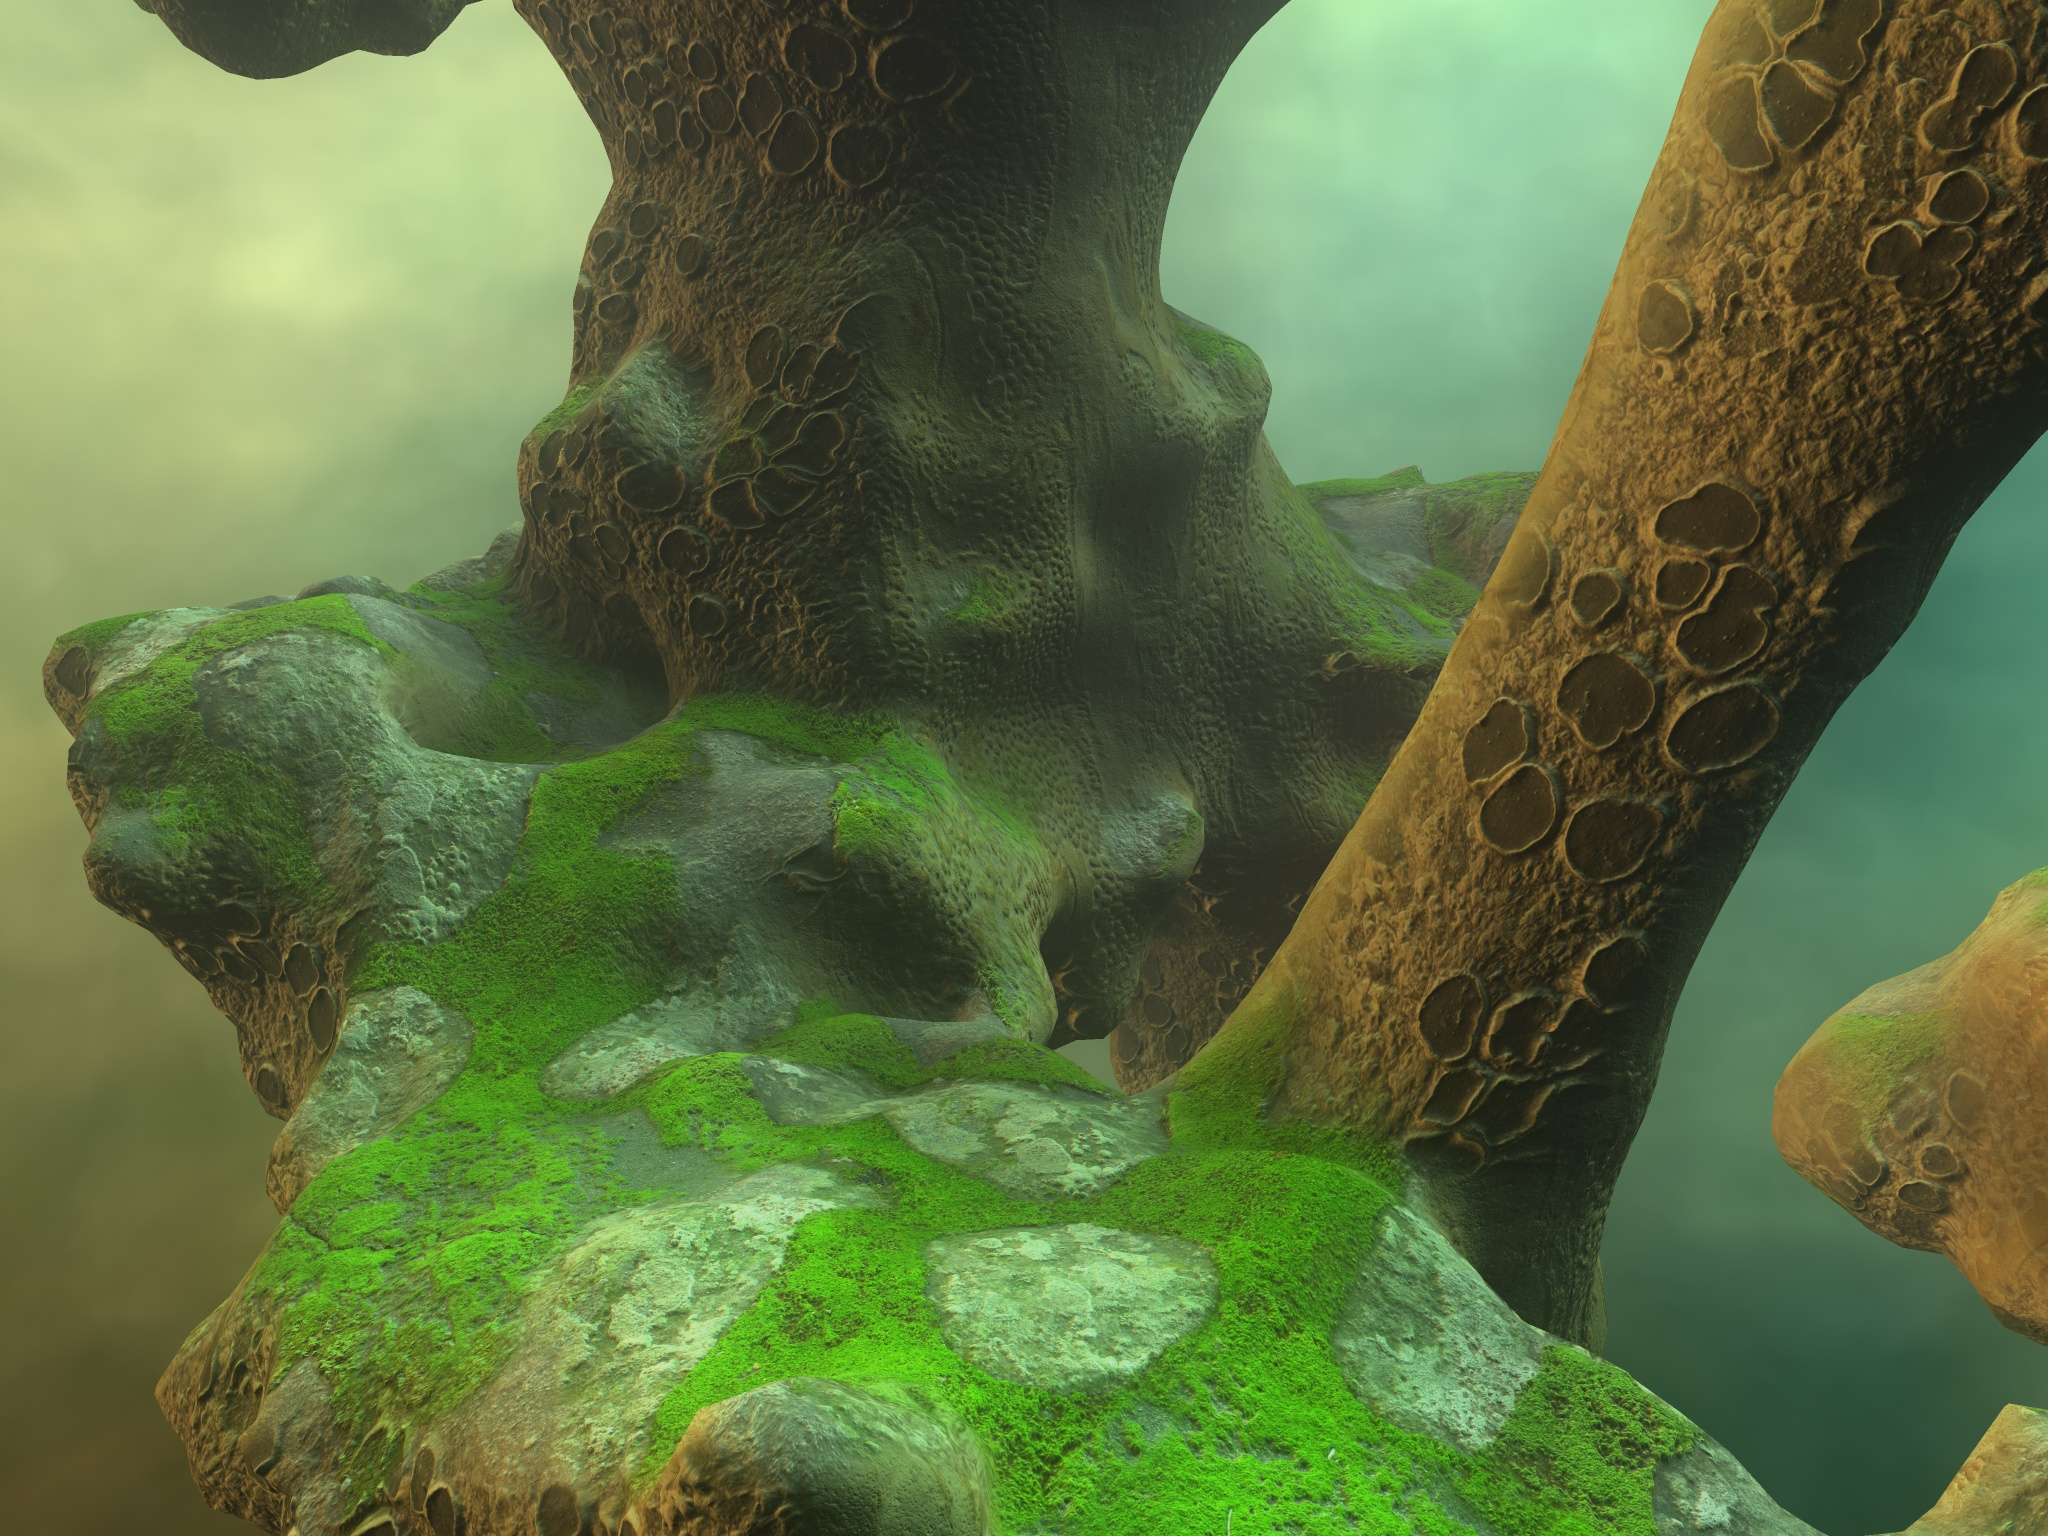
\includegraphics[width=0.5\linewidth]{PICs/cascades}
	\caption{Example of a procedural generated rock. \protect\cite{nvidia::cascades}}\label{cascadesFigure}
\end{figure}

\section{Game Mechanics}
Now it comes to the most crucial part of this chapter of PCG because of its leading part in PCGML as a game mechanic — the use of PCG as a game mechanic! This chapter provides an overview of games which are using PCG as a game mechanic and some examples of possible PCG core mechanics.

\subsection{Current Games} \label{pcgMechanicGames}
Many games are using procedurally generated content in their game nowadays, but not all of them are using PCG as a game mechanic. The following sections describe three games which are using PCG as a game mechanic.

\subsubsection{Galactic Arms Race}
Initially, a research project which is a perfect example of PCG-based core mechanics in a game \cite{game::galacticArmsRace}. Galactic Arms Race is a multiplayer space shooter game in which the player needs to complete tasks and missions to progress through the game \cite{game::galacticArmsRace}. To complete tasks and missions, players need to flight around in space and try to kill enemies with different weapons. A highlight of the game is the particle weapon system which is used to defeat enemies whereas weapons are entirely generated by a PCG algorithm which uses evolutionary AI algorithms to evolve and generate new weapons \cite{pcg::galacticArmsRace}. The AI in Galactic Arms Race creates and evolves weapons based upon actions, strategies, and weapons which are used the most by a player \cite{pcg::galacticArmsRace} \cite{pcg::galacticArmsRace::evolvingContent}. Besides, a player can possess three weapons at a time whereby new evolved weapons are continuously spawned in space and dropped by enemies, and consequently, players need to decide which weapons they want to use and thus feed the AI with information about their preferences \cite{pcg::galacticArmsRace::evolvingContent}. In this case, a player functions as the fitness function of the evolutionary algorithm used by the overall PCG system \cite{pcg::galacticArmsRace::evolvingContent}.\\
In short, a combination of PCG algorithms and evolutionary AI algorithms produces the novel weapon system which represents the core mechanic of Galactic Arms Race.

\subsubsection{Inside a Star-Filled Sky}
Inside a Star-Filled Sky is an almost entirely procedural generated game \cite{game::insideAStarFilledSky}. The objective for a player is to progress through levels and try to reach one of the highest stages of progress to rule the leaderboard \cite{game::insideAStarFilledSky}. Players need to fight enemies, collect items, power-ups or weapons to defeat enemies and get over to the next level. Each level is generated and can represent the inside of an enemy, item or another entity in the game which gives the player an infinite choice of possibilities on how to play the game. Moreover, players can move in or out of the recursively nested levels, and every collected item or killed enemy change the random seed for generating the next level \cite{pcg::endlessWeb}. Players can even move into their character to increase their power and more than 165000 simple weapon combinations are explorable due to PCG \cite{game::insideAStarFilledSky}.\\
Summarized, the core mechanic of Inside a Star-Filled Sky is heavily PCG-based and about exploring and progressing through generated levels with the help of generated weapons and items.

\subsubsection{Endless Web}
Is an entirely PCG-based game and thus uses PCG as its core mechanic \cite{pcg::endlessWeb}. It is about fighting the nightmares in human dreams and rescue the trapped ones and thus releasing dreamers from their fears. The central objective of the game is to rescue six dreamers by exploring the world and make decisions on exploring new areas in the world which affects the parameters of the rescue progress and also the generation of new world parts \cite{pcg::endlessWeb}. For example, if a player kills an enemy then depending on the configuration, it strengthens or weakens an associated challenge and furthermore changes the world \cite{pcg::endlessWeb}.\\
So, Endless Web's core mechanic is about manipulating the generative space where players influence the changes of the world generation with their chosen decisions on how they are playing the game \cite{pcg::endlessWeb}.

\subsubsection{Other Games}
Games like Black \& White, Diablo, Dwarf Fortress, Elite, Eve Online, Roque, Spelunky or Minecraft are other good examples which made use of PCG and related mechanics as an essential part in their game.

\subsection{Possible Core Mechanics}
There are a few possibilities and use cases for PCG as mechanics in games. As seen, some core mechanics aim at weapon creation and progressing through generated space with the help of generated or altered "helper" mechanisms. Apart from that promising ideas are also other noteworthy ideas:
\begin{itemize}
	\item One exciting idea is about using PCG for multiplayer games as a multi-instance PCG system given by \cite{pcg::futureOfPcgInGames}. A game could use a central PCG system consisting of different and unique systems for each player, and every content generation would affect the PCG systems of other players \cite{pcg::futureOfPcgInGames}.  In that case, the core mechanic of the game would include influencing other players with each others PCG system to work towards a specific goal. For example, a use case would be a collaborative multiplayer game where each content generation causes a new content generated in the other’s player space, and they must find a way to communicate how to achieve a mutual objective \cite{pcg::futureOfPcgInGames}. 
	\item There is a lot of research done in the generation of quests as well. The research of \cite{pcg::questGenerator} introduced generated quests based on analysis of four existing \ac{MMORPG} and their quests. One could create a simulation game where players need to create random quests by doing interaction with the PCG system in order to provide an AI agent with missions which needs to be fulfilled to solve some other problems in the game and thus progress throughout the game.
	\item Another idea is to adapt existing and successful introduced game mechanics with a PCG-backend. For example, one could create a game like Tetris where the core mechanics of rotating a block generates new blocks. For example, every time the player rotates the block, the next block will be altered with evolutionary algorithms and changes their shapes to increase the difficulty. Moreover, the system could adapt its difficulty to the player's skills regarding the success or failure rate of using the new blocks to maintain an acceptable experience.
\end{itemize} 

%
% ------------------------------- NEW CHAPTER ------------------------------- %
%
\clearpage
\chapter{\acl{ML}}
\ac{ML} is such a vast topic so that a detailed explanation of every type, approach, method, and model used in ML would go beyond the scope of this thesis. Therefore, the next sections will describe essential subjects of ML which can be useful to understand its further use in PCGML. \\
However, let us ask a question first: What is the difference between ML and AI and what is ML about actually? The fact is, there is no difference between ML and AI. In particular, ML developed from fields of research in AI and is thus a subset of AI. It concentrates on using mechanisms to learn from given data where data represents experience for a given problem. For instance, a famous example of machine learning is an application where the machine can distinguish between apples and pears with the help of a given dataset of features for both apples and pears \cite{ai::book}. 

\section{Types}
Machine learning consists out of three main types which all address a different kind of problem to solve and goal to achieve. One can classify types of supervised learning, unsupervised learning and reinforcement learning \cite{ml::book::developer}. Each of them functions as a solver to a specific task or problem where it fits best and creates the desired results.

\subsection{Supervised Learning}
This type of learning is a task-driven approach of ML \cite{ml::book::developer}. Its primary application is predicting or approximating data based on existing historical or empirical values where the answer to the problem is already known \cite{ai::book}. The previously described problem of classifying apples and pears is a problem is a supervised learning problem which is solved by predicting the specific fruit or also referred as a class \cite{ml::book::developer}. In this case, we would provide a sample set of real data with features for both fruits and classify each feature to a specific fruit. With this, the algorithm links the given features to a specific result and can predict those fruits based on a given test set \cite{ml::book::developer}. A training and test set could exist out of a bunch of pictures or other specific features described with numeric values in a table for each fruit. Hence, the reason why this is called supervised learning is that an ML algorithm is provided with data and therefore knows what to learn \cite{ai::book}.\\
Typical applications for supervised learning are, for example, image recognition and classification, spam detection, pattern detection, speech recognition, \ac{NLP}, sentiment analysis or forecasting \cite{ml::book::algorithms}.

\subsubsection{Regression}
A statistical process is the basis of this supervised learning technique where particular probability distributions of a given training data control the prediction output \cite{ml::book::developer}. In specific, a regression algorithm is processing independent and dependent variables of a given problem and build relationships between them which are furthermore used to predict the correct answers of a given unknown set \cite{ml::book::developer}. Independent variables are describing features and dependent variable the meaning or outcome of a regression problem. Usually, regression algorithms are applicable when the output values are constant prediction problems like for example, the predicted time of completion for a game level based on, e.g., the current player position \cite{ai::book}.\\
Some use cases where concepts of regression algorithms can be applied are, e.g., for imitation and prediction of a player's behavior or player preference learning \cite{ai::book}. Some popularly used algorithm for regression are the linear or polynomial regression, \ac{ANN} or \ac{SVM}. \cite{ai::book}

\subsubsection{Classification}
Addresses problems where classification transition of independent values into specific values is needed \cite{ai::book}. The famous problem of classifying and distinguish apples and pears from each other falls into this section.\\
Like regression algorithms, classification algorithms are applicable for imitation and prediction of a player's behavior, such as prediction of completion time \cite{ai::book}. However, in this case, the possible outputs are specific values or classes like slow, average or fast instead of continuous values \cite{ai::book}. Some popularly used algorithm for classification are, e.g., \ac{ANN}, decision tree, random forests, \ac{SVM}, K-nearest neighbor or ensemble learning \cite{ai::book}.

\subsection{Unsupervised Learning}
In contrast to supervised learning, the base of unsupervised learning is a data-driven approach where the algorithm has no information about the meaning or value of any sample and needs to infer it automatically \cite{ml::book::developer}. Hence, an unsupervised learning algorithm gets so-called unlabeled data without having a specific relationship to the target output and finds unknown structures and pattern in that set \cite{ai::book}. Thinking about the apples and pears example, then an algorithm would try to detect that there are two different types or classes in the dataset instead of predicting if its an apple or a pear.\\
Typical applications for unsupervised learning are object segmentation, similarity or pattern detection, automatic labeling, pre-training of supervised algorithms or pre-processing data such as data compression, noise smoothing or outlier detection \cite{ml::book::algorithms} \cite{ai::book}.

\subsubsection{Clustering}
For example, solves the previous described apples and pears problem by clustering apples and pears out of the given training set with features of both fruits. Based on the trained knowledge due to the training set, it can differentiate new and unknown samples into either apples, pears or an entirely new class \cite{ai::book}. In detail, clustering algorithms are looking for similarities between given features and values, and by doing this, they are inferring a relationship between them and thus separate specific classes \cite{ml::book::developer}.\\
Popularly used algorithms for clustering are, e.g., K-Means, neural networks or \ac{HMM}. \cite{ml::book::developer}

\subsection{\acl{RL}}
In short, \ac{RL} is a goal-oriented approach where an AI tries to reach a goal with the best strategy \cite{ml::book::developer}. RL uses so-called agents who are used to get feedback or specific states of an environment which is further used to learn and improve new decisions based on taken decisions \cite{ml::book::developer}. Inspired by the way humans and animals learn to take decisions, it aims at rewarding the algorithm for good behavior and thus leads it towards the best knowledge and output \cite{ai::book}. \\
In general, RL makes use of a bit of supervision in the form of feedback for an action executed by an agent \cite{ml::book::statistics}. Among experts, this feedback exists as the reward for actions in RL algorithms \cite{ml::book::statistics}.  The tricky part is that RL usually consists of following decisions and every chosen action — chosen out of a set of actions — by an agent is changing the environment which usually makes it difficult to train a model \cite{ml::book::statistics}. Hence, an agent executes different decisions in a loop and is looking for the highest total reward for its sequence of actions since it will always want to increase its total reward. \cite{ai::book} With this strategy, an RL algorithm is getting better and better over time in solving a specific problem until it found the best solution.\\
During the last years, RL algorithms have been used to learn an AI how to play classical games, find the best strategy to win a game, learn an AI how to walk and many other applications \cite{ml::book::algorithms}. Algorithms include neural networks, deep neural networks, Q-Learning or Markov decision process. \cite{ml::book::statistics}

\begin{comment} it doesn't make any sense to describe all learning models for machine learning if they won't be used at all?!
\section{Learning Models}
Which training models are used in ML? --> the 5 tribes of ML\\
"A Machine Learning model is a set of assumptions about the underlying nature the data to be trained for. The model is used as the basis for determining what a Machine Learning algorithm should learn. A good model, which makes accurate assumptions about the data, is necessary for the machine to give good results" \cite{ml:3}\\
each model has its pros and cons and therefore it is not useful to compare each of them without a specific problem or game mechanic problem which should be solved. furthermore, a short description about it as well as pros and cons of their usages shall be given to introduce them. (NO CITE)

\subsection{Linear}
used for regression \cite{ml:2}

\subsection{K-Nearest Neighbor}
used for classification \cite{ml:2}\\
\cite{ml::book::developer} page 72 - 80\\
\cite{ml::book::statistics} page 187 - 202

\subsection{Decision Tree}
\cite{ml::book::algorithms} page >154\\
used for classification \cite{ml:2}\\
\cite{ml::book::statistics} page 119\\
supervised, can be used for either classification, prediction or preference learning tasks. \cite{ai::book}\\
In decision tree learning [67], the function f we attempt to derive uses a decision tree representation which maps attributes of data observations to their target values. The former (inputs) are represented as the nodes and the latter (outputs) are represented as the leaves of the tree. The possible values of each node (input) are represented by the various branches of that node. The goal of decision tree learning is to construct a mapping (a tree model) that predicts the value of target outputs based on a number of input attributes.\cite{ai::book}

\subsection{\acl{SVM}}
\cite{ml::book::algorithms} page >133\\
used for classification \cite{ml:2}\\
\cite{ml::book::statistics} page 214 - 240\\
supervised; alternative and very popular set of supervised learning algorithms that can be used for either classification, prediction or preference learning tasks. is a binary linear classifier that is trained so as to maximize the margin between the training examples of the separate classes in the data (e.g., apples and pears). SVMs have been used widely for text categorization, speech recognition, image classification, and hand-written character recognition among many other areas.\cite{ai::book}\\
Similarly to ANNs, SVMs construct a hyperplane that divides the input space and represents the function f that maps between the input and the target outputs. Instead of implicitly attempting to minimize the difference between the model's actual output and the target output following the gradient of the error (as backpropagation does), SVMs construct a hyperplane that maintains the largest distance to the nearest training-data point of any other class. That distance is called a maximum-margin and its corresponding hyperplane divides the points (xi) of class with label (yi) 1 from those with label -1 in a dataset of n samples in total. \cite{ai::book}\\
They are efficient in finding solutions when dealing with large, yet sparse, datasets as they only depend on support vectors to construct hyperplanes. They also handle well large feature spaces as the learning task complexity does not depend on the dimensionality of the feature space. SVMs feature a simple convex optimization problem which can be guaranteed to converge to a single global solution. Finally, overfitting can be controlled easily through the soft margin classification approach. \cite{ai::book}

\subsection{Neural Networks}
used for regression \cite{ml:2}\\
\cite{ml::book::developer} page >131

\subsubsection{\acl{ANN}}
\cite{ml::book::algorithms} page 289\\
\cite{ml::book::statistics} page 241 - 267\\
supervised, can be used for either classification, prediction or preference learning tasks. but also unsupervised \cite{ai::book}\\
Artificial Neural Networks (ANNs) are a bio-inspired approach for computational intelligence and machine learning. An ANN is a set of interconnected processing units (named neurons) which was originally designed to model the way a biological brain—containing over $10^{11}$ neurons—processes information, operates, learns and performs in several tasks. Biological neurons have a cell body, a number of dendrites which bring information into the neuron and an axon which transmits electrochemical information outside the neuron. The artificial neuron (see Fig. 2.12) resembles the biological neuron as it has a number of inputs x (corresponding to the neuron dendrites) each with an associated weight parameter w (corresponding to the synaptic strength). It also has a processing unit that combines inputs with their corresponding weights via an inner product (weighted sum) and adds a bias (or threshold) weight b to the weighted sum as follows: $x*w+b$. This value is then fed to an activation function g (cell body) that yields the output of the neuron (corresponding to an axon terminal). ANNs are essentially simple mathematical models defining a function $f : x \rightarrow y$. \cite{ai::book}\\
core applications: pattern recogintion, robot and agent control, game-playing, decision making, gesture, speech and text recognition, medical and financial applications, affective modeling, and image recognition \cite{ai::book}\\
pro: compared to other supervised learning approaches is their capacity to approximate any continuous real-valued function given sufficiently large ANN architectures and computational resources. This capacity characterizes ANNs as universal approximators \cite{ai::book}\\
\subsubsection{\acl{CNN}}
\cite{ml::book::developer} page >158
\end{comment}

\section{Development} \label{mlDevelopment}
Developing an easy to use AI needs to be a well-structured and planned process. Especially, when using ML as a focus of interaction, it is even more important to be well-prepared. For this reason, this reason addresses some design considerations about developing user-friendly AI systems in games, as well as standard pitfalls to keep in mind and also possibilities of how to use ML algorithms in two commonly used game engines.

\subsection{Design Considerations}
Someone cannot just develop a new novel AI system and expect to create a whole new experience — it needs to have a thoughtful plan how to achieve new experience \cite{ai::gameDesign}. Firstly, it is useful to think about the MDA framework, which was described in chapter \ref{gameMechanicsChapter}, because an AI-based game is often tightly integrated into its game mechanics and therefore it is necessary to make no mistakes in the first place to fulfill playability and emerging experience \cite{ai::gameDesign}. \\
Here are some critical considerations for AI-based games described by \cite{ai::gameDesign} which are also worth noting for implementing an ML-based AI system: 
\begin{itemize}
	\item First, develop a rough design of the game system and then model the AI system upon that game system or vice versa \cite{ai::gameDesign}. In particular, for AI-based games, the AI system should support the designed core experience of the game \cite{ai::gameDesign}.
	\item An AI should provide possible exploration and allow a player to experiment with it which means it should be robust enough and not lead to game crashes or misbehavior \cite{ai::gameDesign}. 
	\item Avoid a too mechanical and unnatural player experience with an unpredictable system \cite{ai::gameDesign}.
	\item The environment of an AI-based game should be observable for an AI system which means it should be able to access states of different game entities at any time \cite{ai::gameDesign}. Consequently, game states should be described in a way so that an AI system can easily access and read it \cite{ai::book}.
	\item A system should be as accessible and transparent as possible for a player so that a player will not be overwhelmed by the system and its possibilities \cite{ai::gameDesign}. Notably, an interactive ML system as an AI system in the game could be a confusing thing for a player if it, e.g., exposes too much information \cite{ai::gameDesign}. That is of particular importance when using \ac{RL} as the backbone AI agent algorithm.
	\item Provide ways for emergent gameplay with the help of the AI system with, e.g., possible strategies which can be applied to the system \cite{ai::gameDesign}. 
\end{itemize}
Lastly, the discussed issues and considerations in chapter \ref{mechanicsConsiderationsPCGandML} also apply for the implementation of an ML-based AI agent.

\subsection{Common Pitfalls}
Following pitfalls are commonly occurring problems when implementing and training machine learning models for a specific problem.

\subsubsection{Under- and Overfitting}
ML models are used to approximate unknown output based on given training data \cite{ml::book::algorithms}. When talking about fitting, then it is referred to fit a model to a given training set and its features which are used to train the model. This set can consist of many independent variables and different entries which can create some issues:
\begin{itemize}
	\item \textbf{Underfitting}: Happens when the training set for the model consists of too less information or independent variables \cite{ml::book::algorithms}. In that case, the model is not able to capture the dynamics of the values \cite{ml::book::algorithms}.
	\item \textbf{Overfitting}: Is exactly the opposite of underfitting. When a model is over-fitted then it is fed with too much information and variables so that it is not able to generalize the dynamic relationship of variables during the training \cite{ml::book::algorithms}.
\end{itemize}
Therefore, a right amount of information for the training of a machine learning model should be provided to achieve an excellent fitted model. A method to check and prevent the model from being over or under-fitted is the technique of validation such as cross-validation which helps to detect those problems \cite{ml::book::algorithms}.

\subsubsection{Curse of Dimensionality}
This problem often occurs when the training set is smaller than the number of feature variables, or also called the dimensions of a set, which are used to train a model \cite{ml::book::algorithms}. In this case, if the number of features increases then the performance of the model gets dramatically reduced \cite{ml::book::algorithms}. Possible ways to prevent and solve this problem are, e.g., a decrease of dimensions or providing more training data \cite{ml::book::algorithms}.

\subsection{Game Engine Plugins}
Indeed, all the different machine learning models or the one which applies to the game prototype of this thesis could be self-implemented. However, there are other people out there who have already implemented and improved their implementations which are a good starting point when implementing a PCGML game mechanic. As discussed at the beginning of the thesis, it is going to focus on an implementation in commonly used game engines which is the reason why to envisage the two most used free to use game engines nowadays.

\subsubsection{Unity}
Unity made an incredible effort in its research and use of machine learning in their engine in the last year \cite{unity::ml}. They recently released a beta version of an open-source ML agents plugin that enables games to train an AI with \ac{RL}, imitation learning, neuroevolution or other ML methods \cite{unity::mlGithub}. The base of the plugin is Google’s open-source ML framework TensorFlow \cite{api::tensorFlow} which is accessible via a simple-to-use Python \ac{API} \cite{unity::mlGithub}. They are also providing essential instructions and documentary for the usage of their plugin which is a promising, definite and significant advantage when implementing the PCGML game mechanic.

\subsubsection{Unreal Engine 4}
At the time of writing this section, there is no available officially announced ongoing plugin or feature development for ML in \ac{UE4}. However, there are others who were concerned about the missing feature of ML in UE4. For this reason, \cite{ue4::tensorFlowPlugin} created an open-source TensorFlow plugin for UE4 which implements a Python API accessible interface. Indeed, there are also some other plugins available via UE4's marketplace such as a Q-Learning plugin, but there do not look that promising as \cite{ue4::tensorFlowPlugin}'s TensorFlow plugin. Also, provided documentation and guidance on how to use the plugin leads it to a tolerable option besides to Unity’s ML agent plugin.

\section{Game Mechanics}
It is unclear which games used specific methods of ML for a game mechanic because there are not any research paper or published articles about, i.e., game companies who talked about using ML for their mechanics. Nevertheless, there is a research focus on AI-based games, including game mechanics which can be adapted with ML and is therefore used to come up with ideas for ML game mechanics. 

\subsection{Current Games}
Two games which use AI as a core mechanic were already described in chapter \ref{pcgMechanicGames} and are the games Endless Web and Galactic Arms Race. Both making use of a PCG and AI mixture mechanic where the AI generates new world segments based on game world states \cite{pcg::endlessWeb} or new weapons based on player preferences \cite{pcg::galacticArmsRace}. These games are going to be first reference points and inspiration when implementing a PCGML game mechanic. Other games which used ML techniques as a mechanic were, e.g., Black and White and Creatures \cite{ml::mostInfluentalAiGames}. 

\subsubsection{Black and White}
The player is in control and owns a creature who can be trained to do things for the player. They used techniques such as decision trees and neural networks to train and learn it the prediction of a player's action \cite{ml::gamasutra::ml} \cite{ml::mostInfluentalAiGames}. In particular, the belief-desire-intention approach was used to implement the creature's behavior \cite{ml::mostInfluentalAiGames}. The creature's training happens due to a player’s reaction upon the creature's executed actions which therefore follows the rules of RL where the creature would like to achieve the best total reward for its behavior \cite{ml::gamasutra::ml}.

\subsubsection{Creatures}
That is a game where players need to hatch animals and try to teach them how to behave and survive in their world \cite{ml::mostInfluentalAiGames}. As well as Black and White, Creatures also used neural networks to teach and learn animals how to behave based on a player's input \cite{ml::mostInfluentalAiGames}.

\subsection{Possible Mechanics}
\cite{ai::aiBasedGameDesignPattern} introduced nine design patterns, summarized in Table \ref{AI-basedMechanicsDesignPattern} which illustrates ways to develop game mechanics based on AI techniques and furthermore to create AI-based games. Following sections describe some examples of possible mechanics or core mechanics with ML, based on \cite{ai::aiBasedGameDesignPattern}'s design patterns.
\begin{table}[!htbp]
	\centering
	\resizebox{\textwidth}{!}
	{%
		\begin{tabular}{|p{2.1cm}||p{8cm}|p{4cm}|p{4cm}|}
			\hline
			\multicolumn{1}{|c||}{\textbf{Pattern Name}} & \multicolumn{1}{c|}{\textbf{Description}} & \multicolumn{1}{c|}{\textbf{Role of Player}} & \multicolumn{1}{c|}{\textbf{Role of AI}} \\ \hline\hline
			\textbf{Visualized} & Visualization of AI system states so that gameplay revolves around state manipulation & Observation and manipulation of an AI system & Shows states and gives information \\ \hline
			\textbf{Role-Model} & Player needs to imitate AI agents & AI system imitation & Shows actions and behavior, e.g., as a puzzle \\ \hline
			\textbf{Trainee} & AI system needs to be trained to perform gameplay tasks & Teacher for AI system & Learns desired behavior \\ \hline
			\textbf{Editable} & Player needs to change elements of an AI agent which are related to gameplay & Observation and manipulation of the AI & Handles changes and shows a new behavior \\ \hline
			\textbf{Guided} & Player partly assists or guides an AI agent who is threatened  by a problem & Guidance and management of the AI & Acts on its own but mostly does what the player wants \\ \hline
			\textbf{Co-Creator} & Player and AI work together as equal partners & Learns how to play the game with AI assistance & Acts as co-creator and assistance for the player \\ \hline
			\textbf{Adversary} & Player needs to defeat an AI system & Adapts to an AI and defeats it & Tries to defeat the player \\ \hline
			\textbf{Villain} & Player needs to defeat an AI system whereas AI system does not want to defeat the player & Adapts to an AI and try to defeat it & Acts as villain and mob the player \\ \hline
			\textbf{Spectacle} & AI which implements a complex system and the player needs to observe, interact or overcome it & Observation, interaction or manipulation of the system & Spectacles and simulates the system \\ \hline
		\end{tabular}%
	}
	\caption{AI-based game mechanics design pattern \protect\cite{ai::aiBasedGameDesignPattern}}
	\label{AI-basedMechanicsDesignPattern}
\end{table}

\subsubsection{AI as Role-Model}
For example, a game in which a player needs to follow an AI to solve quests or missions. Based on the players progress in each quest and imitation level, the AI adjusts its solution of solving the current or a new problem and provides the player with either a less competitive or harder solution and reward. Hence, player experience is adapting due to player behavior learning and predicting an appropriate difficulty level. For instance, a quest could be following or remembering the path of the AI to a treasure whereas built-in traps are crossing the way. Hypothetically, if the player cannot remember and succeed the path after, e.g., three times, then the AI shows a new and less challenging path to a less rewarding treasure.

\subsubsection{AI as Trainee}
Is one of the most promising design pattern since it revolves around teaching an AI different things whereby it fits perfectly for using ML methods. As introduced before, the games Black and White and Creatures are using precisely this kind of pattern for implementing their creature behavior. A game could use a mechanic like the same and introduce new mechanics on how to interact and use the AI agent by teaching it how to behave in specific situations. A simple idea would be a teaching game in which the player needs to educate fighters to defeat enemies. Alternatively, a tower defense game in which the player uses defense entities to teach an ML agent first target preferences.
	
\subsubsection{AI as Co-Creator}
An exciting base idea of a co-creator AI game would be a split-screen game in which the player plays on one side and the AI agent on the other side. The gameplay would be symmetrical, and everything a player does will be tried to imitate by the AI. In doing so, the player needs to do things to complete challenges whereas done actions affect the AI agents space and vice versa. For example, a challenge could be pushing a button which only exists in the space of the AI but opens, e.g., a door in the player's space. Therefore, the player would need to behave in a specific manner to lead the AI towards the button to progress through the game.

%
% ------------------------------- NEW CHAPTER ------------------------------- %
%
\clearpage
\chapter{\acl{PCGML}}
A purpose for research in AI-based PCG methods like PCGML was to invent algorithms which are able to create and generate content of the same type and style based on existing content with or without human involvement \cite{ai::book} \cite{pcgml::paper}. In general, \cite{pcgml::paper} defined PCGML as ''the generation of game content using machine learning models trained on existing content''. \\
On this account, different research was and is going on to generate music, sound effects, images, textures, worlds or levels \cite{ai::book}. Research showed that ML-based PCG methods are working well for music and images types but are facing some issues when it comes to world or level generation because of its necessity of playability to create an experience \cite{ai::book}. Thus, the generation of gameplay connected game content pointed out some challenges which further research is going to address and try to solve \cite{ai::book}. It is for this reason why PCGML approaches were not used in games yet. Another reason is that there is often not enough game content available to train a PCGML model on for a specific content generation problem \cite{ai::book}. \\
The next chapters introduce the difference to usual PCG, use cases of PCGML and some developmental features used in other research. Overall, this chapter is not going into many details since all essential cornerstones of PCGML where discussed and introduced in the previous chapters.

\section{Difference to \acl{PCG}}
What usual PCG and PCGML have in common are their hand-made algorithms, parameters, and constraints made by developers \cite{pcgml::paper}. Typically, designers would use existing game data and content to get inspired by and create generators which can generate new material on top of that inspiration whereas PCGML itself can get inspired by existing data to develop new content and thus assist the designer \cite{pcgml::paper}. So, the basic idea is to train the PCGML model on various game content and produce new content \cite{pcgml::paper}. \\
In contrast, different PCG algorithms might use ML for evaluation, but their content generation process entirely relies on their specific domain space rather than a trained model space \cite{pcgml::paper}. For example, experience-driven PCG relies on models of player experience whereas PCGML models can use preference or behavior learning to create new content \cite{pcgml::paper}.

\section{Use Cases}
The focus of PCGML is to generate new content based on training with existing content. For this reason, PCGML can be used mainly for adaption, reparation, evaluation, critique or analysis of new content but also for general PCG tasks like autonomous generation, co-creative, and mixed design or data compression \cite{pcgml::paper}.
\begin{itemize}
	\item \textbf{Autonomous Generation}: Is one of the primary applications for PCGML because it can generate game content without human input which is especially useful when online content generation is needed \cite{pcgml::paper}. Also, a designer could create, e.g. a set of levels and feed the model with these models in order to create new and novel but similar levels with the help of the PCGML system \cite{pcgml::paper}.
	\item \textbf{Co-creative and Mixed-initiative Design}: This use case focuses on the collaboration between designers and the PCGML algorithm \cite{pcgml::paper}. For instance, the algorithm could generate new content based on existing provided content as a draft for the designer who could polish and finish the drafted content afterwards.
	\item \textbf{Data Compression}: PCGML offers significant potential for data compression with the help of ML. By extracting specific dimensions of game content can save data size and would allow more efficient storage \cite{pcgml::paper}.
	\item \textbf{Recognition}: This is where PCGML stand out from the usual PCG algorithms. Its capability use of recognition makes it possible to analyze, evaluate, adapt, critique or repair either existing, new designed, player created or algorithm generated game content \cite{pcgml::paper}. 
	\item \textbf{Repair}: In particular, reparation of a designed or generated content can be a useful tool. For example, during generation or learning time, the algorithm could check for, e.g. playability of a level and repair it immediately or suggest a fix \cite{pcgml::paper}.
\end{itemize}

\section{Development}
{\color{blue}There are no specific development considerations to make when someone uses the combination of PCG and ML. Instead, every design consideration, possible issue, pitfall and best practices described and discussed in chapters \ref{pcgDevelopment} and \ref{mlDevelopment} will apply when implementing PCGML algorithms.\\
Nevertheless, it is worth mentioning that commonly used training models for research purposes, e.g., by \cite{pcgml::paper}, were:
\begin{itemize}
	\item Neural networks like \ac{ANN}, \ac{CNN} or \ac{LSTM} networks
	\item Markov models such as n-grams or multi-dimensional Markov chains
	\item Bayes models
	\item Autoencoders
	\item Clustering
	\item Matrix factorization
\end{itemize} 
}


\subsection{Data Representation}
{\color{blue} Needs to be addressed! Pick one of the representation used in the PCGML paper and describe it in a summary.}

\begin{comment}
%
% ------------------------------- NEW CHAPTER ------------------------------- %
%
\clearpage
\chapter{\acl{PCGML} Game Mechanics}
the design process for \cite{pcg::endlessWeb} followed the principles of \cite{ai::gameDesign} with Launchpad as the AI system.

\section{First Considerations}
\end{comment}

\section{Concepts of Possible Game Mechanics}
The initial ideas on how to use PCGML as a game mechanic were created by \cite{pcgml::paper}. They came up with seven different ideas which were based on the AI-based game design pattern from chapter \ref{AI-basedMechanicsDesignPattern}:
\begin{itemize}
	\item \textbf{Role-Model}: "A \ac{PCGML} system replicates content which is generated by players of various levels of skill or generates content suitable for players of certain skill levels. New players are trained by replicating the content or by playing the generated content in the form of generative tutorial." \cite{pcgml::paper}
	\item \textbf{Trainee}: "The player trains a \ac{PCGML} system to generate a piece of necessary content (e.g., part of a puzzle or level geometry)." \cite{pcgml::paper}
	\item \textbf{Editable}: "Rather than training the AI to generate the missing puzzle piece via examples, the player changes the internal model’s values until acceptable content is generated." \cite{pcgml::paper}
	\item \textbf{Guided}: "The player corrects the \ac{PCG} system’s output to fulfil increasingly difficult requirements. The \ac{AI}, in turn, learns from the player’s corrections, following the player’s guidance." \cite{pcgml::paper}
	\item \textbf{Co-Creator}: "The player and a \ac{PCGML} system take turns in creating content, moving towards some external requirements. The \ac{PCGML} system learns from the player’s examples." \cite{pcgml::paper} 
	\item \textbf{Adversary}: "The player produces content that the \ac{PCGML} system must replicate by generation to survive or vice versa in a “call and response” battle." \cite{pcgml::paper}
	\item \textbf{Spectacle}: "The \ac{PCGML} system is trained to replicate patterns that are sensorically impressive or cognitively interesting." \cite{pcgml::paper}
\end{itemize}
This ideas were used to come up with more ideas on how to use PCGML as a game mechanic in modern video games.

\subsection{Rules and Behavior} \label{idea::rulesAndBehavior}
A possible idea is a PCGML system which generatee rules for a strategy game. A generic and modular strategy game offers the perfect foundation for generating its internal rules and behavior based on its internal elements. In particular, a strategy game mostly exists out of different sequences of actions emerging from new elements in the game which furthermore lead the game in a specific direction. All of those available actions have a different effect in the game whereas the effects can be changed with other appropriate effects causing different changes during the game. Especially, the design of a strategy game can introduce more possible usable game elements than used in the game itself. This kind of game element preselection often arises in card board games where players need to choose the available cards in advance which affects the flow of the game. For example, if a game provides the players with 25 different elements and just 10 element are used in the game, then it provides, regarding the mathematical theorem of combinatorics, 3268760 possible ways to play a game. This formula only applies if each element will be introduced after a specific time and can't be reused. Moreover, specific conditions for, e.g, the specific timeslot in which a element will be releaved can also be a part of the generation process which emerges a more dynamic game.\\
In this case, the training of the PCGML system is based on working configurations of the game in which it learns the different dependencies between elements and effects to each other. 

%$ \dfrac{N!}{n!(N-n)!} = \dfrac{25!}{10!15!} = 3.268.760 $

\subsection{Changing Weapons} \label{idea::changingWeapons}
Game mechanics are often related with some kind of interactable objects. In the case of a \ac{FPS} game, these objects are represented by different weapons like guns, rifles or shotguns where often other mechanics such as particular tactics evolve as a result. With this in mind, another idea of using PCGML as a game mechanic is its use as any kind of weapon generator. In specific, an FPS game with generated weapons where providing different weapons at the training time results in different ways to play the game. A virtually created weapon can have different properties, such as weight, blowback power, firing rate, ammunition and others which form the base to procedurally generate new weapons. Furthermore, as weapons need ammunition, the generation of novel bullets and projectiles can also be part of the PCGML system. \\
For example, a game could be a FPS game with generated weapons from a pretrained PCGML system whereby the model will be fed with the new generated weapons during runtime and furthermore specializes in a specific direction. After a bunch of time, the system only generates a specific weapon and that is where the game or session would end.

\subsection{Changing Powers} \label{idea::changingPowers}
Often, the main mechanic provided in most \ac{RPG} is fighting with a sword, any kind of weapon or applying magic spells as an attack to the enemy. Moreover, the weapons often possess a magic power as advantage or disadvantage. These powers and the magic spells themselves can be part of a generation process powered by a PCGML system. The system could generate new weapons or spells affecting the duration, spell category, continuing effect on the enemy or player, energy cost and other similar and often used properties. Training of the system would be done with providing useful weapons with advantages or disadvantages or some magic attacks as an example.

\subsection{Solver Weapon} \label{idea::solverWeapon}
This is an idea based on the co-creator pattern described in chapter \ref{AI-basedMechanicsDesignPattern}. It is about a game mechanic of using a generation weapon to progress through the game. Its purpose it to help the player in special conditions such as solving puzzles with a missing piece in it. The highlight of the game mechanic is the required drawing interaction to generate a missing piece. A player needs to draw the missing piece on a given "drawing panel" connected with the weapon which tries to replicate the figured piece. Drawings could consist of fat circles indicating corners and lines representing edges. The detection of the drawing involves object detection via ML which forwards detected chunks to the PCGML system. For example, an introductory gameplay could be to find or generate the missing key for a door whereas the shape of the lock is shown to the player.\\
This idea could work as follows: 
\begin{enumerate}
	\item The ML part is trained on different input with different drawing of puzzle elements or geometric shapes depending on the style. The system is then able to detect important points on the drawing and suggests what the drawing would be.
	\item The PCGML system detects the drawings with any kind of object detection algorithm. As the system has obtained the chunks of the detection algorithm, it uses each chunk data to generate a fragment of a geometry and finally combines all of them into a combined shape.
\end{enumerate}
Furthermore, this idea can be extended with the trainee and guided pattern where the player would provide the system with feedback if the PCGML system outputs the wrong object. In this case, it would learn the specific drawing conventions of a player and adjust itself to the player.

\subsection{Defeat of the Enemy} \label{idea::defeatTheEnemy}
The PCGML system tries to defeat the player and one or more players try to defeat the enemy. This is based on the adversary design pattern described in chapter \ref{AI-basedMechanicsDesignPattern} where the role of the AI is to defeat the player. In this case, the system is trained on simple player behavior such as movement paths or attack  preferences in a specific environment and uses this knowledge to overcome the player. Moreover, it would be also able to find new behavior pattern during the fight. Summarized, the output of the system are new tactics, behaviors or attack sequences for the AI on how to defeat a player. Furthermore, the PCGML system could categorize used behavior regarding their success or failure and learn from these outcomes to increase its accuracy. \\
An example scenario would be that an AI has the intention of applying a critical hit to the player. In doing so, the PCGML system generates, e.g., a possible path to fulfill the desire of hitting the player based on, e.g., both the players and AI positions and the pretrained knowledge.

\subsection{Caught in a Thunderstorm} \label{idea::caughtInAThunderstorm}
A game which revolves around a player which is in control of a thundercloud and has the objective to destroy cities or enemies with the power of lightning. In this scenario, a PCGML system would generate pattern for the diffusion of lightning and impact points based on different weather conditions, cloud height, enemy or building position, physical materials and similar properties. This idea offers its potential as a thunderstorm simulation game which is based on empirical or real data of weather which is used to train the PCGML system.

\subsection{Train to Progress} \label{idea::trainToProgress}
A player is provided with a completely empty and untrained PCGML system. The system is able to generate an important part for the gameplay but needs to be trained first to activate its full functionality of generating necessary or missing elements. In this case, a player's main objective is to train the PCGML system to progress towards a given goal. For instance, a puzzle game where the main puzzle is the system's training to generate, e.g., some missing piece. A level could contain hidden objects which needs to be found first to properly train the system. \\
For example, if the objective would be to unlock a locked door with a generated key then the player needs to find sample keys first to train the system with those which are similar to the locks key. If there isn't any success in generating the right key then the player can reset the systems internal model and try it again with another pair of sample keys. This principle also offers its application with other kinds of objects and is mainly based on the trainee design pattern.

\subsection{Building with Assistance} \label{idea::buildingWithAssistance}
Revolves around a PCGML system, trained to generate incomplete game elements for a specific goal. For example, a building game where the PCGML system never outputs the correct element which is currently needed. On the other hand, the player has the abilities to improve and overhaul the generated elements. All changes will be then fed into the system which guides its internal model to a desired generation output direction. Thus, this idea is heavily  based on the guide design pattern with the focus on guidance. The training of the PCGML system would consist of examples of incomplete but usable and modification able game elements.

\subsection{The exploring Co-Worker} \label{idea::exploringCoWorker}
Another idea based on the co-creator pattern could be, e.g., a strategy game where the player's focus is to mine, build and create strategic plans to overcome its opponent. Moreover, in order to evolve in the game, the player possesses a PCGML system which is used to explore and conquer new sections of a map. This system would work completely on its own and just functions as a helper and teammate for the player. The exploration process of a new section consists basically of creating new terrain by the system. In this case, the system is trained to generate new chunks or section of unexplored terrain mainly based on the player's progress, mined resources and similar elements.

\subsection{Observe and Learn} \label{idea::observeAndLearn}
A PCGML system which is trained to generate and modificate terrains with a special path within the terrain to reach a certain goal. The highlight is that the system doesn't always generate possible ways which demands the player to change properties of the system which changes a terrain, the level, map or world. In doing so, the player is forced to observe the interactive and smooth changes of the system to reach the current goal. This idea is based on the visualization and editable design pattern.

\subsection{Express Yourself} \label{idea::expressYourself}
An application as a game mechanic in a point and click game could be a PCGML system, trained to generate new storylines, events, choices and outcomes of chosen choices. The system is trained on existing designed stories and learns the dependencies to create new and novel storylines which individual possible choices and outcomes. Like in the idea described in  \ref{idea::rulesAndBehavior}, the designer can provide more game elements than actually used in the game which provides the system which a various of possibilities on how to compose the game. This idea of a PCGML generated story is mainly based on the spectacle pattern.

\subsection{Big Boss Helper} \label{idea::bigBossHelper}
This idea is based on the villain pattern in which the AI just mobs a player rather than tries to defeat them. This kind of design pattern fits almost perfectly in, e.g., a big boss fight with more than one NPC to defeat as it is often used in RPG games. For example, there are two NPC's to defeat to win the fight and obtain special items - one applies mainly damage and the other one protects the other one. This helper NPC is represented by the PCGML system which is trained on player behavior such as attack preferences or movement behavior in a specific level or environment to generate or alter the terrain or level to keep the player off the main enemy in the fight.

\subsection{Figure it Out} \label{idea::figureItOut}
A possible application in a multiplayer game could be a mechanic in which each player possesses a PCGML system for generation purposes. But the challenge in the game is that each generation of the system changes the other's systems output and they need to work together towards a specific goal. For instance, a puzzle game where players need to figure out the connection between their system. The PCGML system would be trained with a specific game corpus and enables interaction based on the editable pattern. The player changes parameters and also changes the other while they need to generate an object combined with each of the systems output. Parameter adjustment can either be done directly or indirectly with any kind of minigame like moving stones around in a room and find the right position. Furthermore, this idea can also be used in a single player puzzle game without the need of another player.

\subsection{Novel Vehicles} \label{idea::novelCars}
Another possible field of application for a PCGML system can be the generation of cars or vehicles as they also consist of many properties and parameters. The process of finetuning of these properties is usually a long process which is a perfect field of application for a ML trained PCG system.

\section{Development Evaluation of Concepts}
The main issue in the implementation of the PCGML system will be the training data for the ML model rather than the PCG output itself. A proper training for the ML model requires the right amount of training data to function as intented (CITE?). The size of the dataset can differ from application to application based on the given values as dependencies for an output (CITE?). Following chapters evaluate each game mechanic based on their pros and cons for a possible implementation. In particular, each idea has the advantage of PCGML that it can generate similar elements as used during training time, possibility of changing the training set and thus the output and also no need of finetuning to generate a broad range of elements in contrast to standard PCG algorithms. For this reason, as it is the implication of using PCGML, these described advantages are not mentioned in the evaluation. Also, the provision of playability is a necessary thing which contributes equally in each game mechanic.

\subsection{\nameref{idea::rulesAndBehavior}}
\textbf{Pros:}
\begin{itemize}
	\item A proper learned model can be saved to generate the same sessions again.
	\item Providing more designed content in the training set offers more possibilities for the gameplay.
\end{itemize}
\textbf{Cons:}
\begin{itemize}
	\item Need a complex game design with dependencies between usable elements.
	\item Possible complications in the training of the ML model because elements can consist of many values which create complex dependencies.
	\item Game design must include a broad range of game elements with harmonization between each other and proper design and balancing.
\end{itemize}

\subsection{\nameref{idea::changingWeapons}}
\textbf{Pros:}
\begin{itemize}
	\item Open source FPS projects are offering a good base of training data to work on.
	\item Properties of weapons and ammunition are not quite complex to train the ML model.
	\item It does not matter if the generated weapon works in every environment. Different weapons offer different advantages in different environments.
	\item No need of complex game design.
\end{itemize}
\textbf{Cons:}
\begin{itemize}
	\item Diversity of weapons can be minimal if not enough weapons are represented because of the non complex structure.
\end{itemize}

\subsection{\nameref{idea::changingPowers}}
\textbf{Pros:}
\begin{itemize}
	\item Magic attacks and spells do not need to be effective because their tactical use forms their effectiveness in the game.
	\item There are no general rules of what and how spells and magic attack appear in games, thus they can be anything.
	\item Do not often consist of complex structures  which should make ML model training easy.
\end{itemize}
\textbf{Cons:}
\begin{itemize}
	\item It needs a good design of balanced and tweaked spells.
	\item Visuals should also be part of the generation process otherwise it looks odd.
\end{itemize}

\subsection{\nameref{idea::solverWeapon}}
\textbf{Pros:}
\begin{itemize}
	\item Training set for each models can be easily created.
	\item Concept is straight forward and easy to learn.
	\item \ac{VR} offers easy-to-use drawing mechanic.
\end{itemize}
\textbf{Cons:}
\begin{itemize}
	\item It needs two trained ML models - one for the object detection and another for the generation of puzzle objects. 
	\item Needs design of proper puzzles where mechanic is used with generated objects.
\end{itemize}

\subsection{\nameref{idea::defeatTheEnemy}}
\textbf{Pros:}
\begin{itemize}
	\item Training input for ML model can be real data of fights with a standard AI enemy, extended with randomized values.
	\item Possible improvement of ML model during runtime with system feedback.
\end{itemize}
\textbf{Cons:}
\begin{itemize}
	\item PCG generation and especially interactive modification of terrain can be complex.
	\item Needs good balanced training set to not overwhelm the player with a too hard enemy.
\end{itemize}

\subsection{\nameref{idea::caughtInAThunderstorm}}
\textbf{Pros:}
\begin{itemize}
	\item Pattern generation is easy to implement with, e.g., L-system.
	\item Training of ML model is possible with statistical, empirical and real data.
\end{itemize}
\textbf{Cons:}
\begin{itemize}
	\item Needs a proper game design with a sense for the mechanic.
	\item The proper simulation of weather conditions and changes can be complex to implement.
\end{itemize}

\subsection{\nameref{idea::trainToProgress}}
\textbf{Pros:}
\begin{itemize}
	\item The ML model does need pretraining because it is done in the game by the player.
	\item Creation of puzzles do not need to consider PCGML system because the system is based on the puzzle.
\end{itemize}
\textbf{Cons:}
\begin{itemize}
	\item It takes a time to properly train the model by the player and it can be frustrating if the model does not learn properly.
	\item Each puzzle element needs own design and own PCGML system.
\end{itemize}

\subsection{\nameref{idea::buildingWithAssistance}}
\textbf{Pros:}
\begin{itemize}
	\item PCG is easy to implement since it just needs to generate objects proper to the game corpus.
	\item There is a margin for generation errors because it revolves around guidance of the PCGML system.
\end{itemize}
\textbf{Cons:}
\begin{itemize}
	\item The generation of usable and extendable elements need to be secured.
	\item The model takes a while to get properly guided it can be frustrating if nothing right is generated in the beginning of the game.
	\item Needs a interaction system with generated objects.
\end{itemize}

\subsection{\nameref{idea::exploringCoWorker}}
\textbf{Pros:}
\begin{itemize}
	\item PCGML implementation focuses only on the exploring task.
	\item Terrain generation can be based on the game corpus and does not apply to special rules. Thus, training of the ML model with sample terrains should be easy.
\end{itemize}
\textbf{Cons:}
\begin{itemize}
	\item PCG generation and especially interactive modification of terrain can be complex.
	\item Terrain needs to be interactable with the player's mechanics to build and mine.
\end{itemize}

\subsection{\nameref{idea::observeAndLearn}}
\textbf{Pros:}
\begin{itemize}
	\item Terrain generation can be based on the game corpus and does not apply to special rules. Thus, training of the ML model with sample terrains should be easy.
	\item There is a margin for errors since it is the system conception to work faulty and the player's task to interact with the system to reach the goal. 
\end{itemize}
\textbf{Cons:}
\begin{itemize}
	\item PCG generation and especially interactive modification of terrain can be complex.
	\item Necessity of "incorrect operation" for challenging terrain generation needs to be secured.
\end{itemize}

\subsection{\nameref{idea::expressYourself}}
As described in the first idea about rules and behaviors, the same type of considerations apply for this idea about generating whole storylines with interaction.

\subsection{\nameref{idea::bigBossHelper}}
The same pro and cons described for the mechanic "\nameref{idea::defeatTheEnemy}" applies for this concept since their PCGMl systems are operating in the same manner.

\subsection{\nameref{idea::figureItOut}}
\textbf{Pros:}
\begin{itemize}
	\item Creation of puzzles do not need to consider the PCGML system because the system revolves around the puzzle.
	\item Training of the ML models should be easy since they are based on a puzzle. Thus, the PCG should be easy to implement.
	\item Each PCGML system focuses on their own piece of the puzzle element.
\end{itemize}
\textbf{Cons:}
\begin{itemize}
	\item It needs training for each ML model and puzzle.
	\item Each puzzle element needs own design and own PCGML system.
	\item The connection between PCGML systems will be complex, therefore it needs a good design of the system's connection.
\end{itemize}

\subsection{\nameref{idea::novelCars}}
\textbf{Pros:}
\begin{itemize}
	\item Generated vehicles can decide the kind of game where it is used, therefore it does not matter what is output as long it secures playability.
	\item Vehicles are not limited to cars, therefore it can be any kind of driveable vehicles.
\end{itemize}
\textbf{Cons:}
\begin{itemize}
	\item The training set needs the designs of a lot of vehicles, so the system can learn the complex dependencies of a vehicle.
	\item The design of vehicles often involves a long process of balancing.
\end{itemize}

\section{Summary}

Of course, the generation of any kind of item, quests, missions or challenges is also possible with PCGML. Or the implementation of any kind of progression mechanics can be done via PCGML. One just needs to figure out the important properties of the generating element to train the ML system properly.

A summary of each PCGML game mechanic training data and output can be found in appendix \ref{gameMechanicIdeaSummary}

\subsection{Game Mechanic for the Prototype}
what is the best game mechanic? why? etc


%
% ------------------------------- NEW CHAPTER ------------------------------- %
%
\clearpage
\chapter{Game Prototype}
Development of a game with one of the best-evaluated PCGML game mechanic as the central game mechanic of the game.
\section{Considerations}

Evaluation of PCGML hardware and software requirements
\subsection{Which Game Engine?}
There are 2 main engines which are commonly used thorough the industry due to their fact of free to use.

\subsection{Which Learning Model?}
state different models which could be used and differ them

\section{Game Design}
\begin{itemize}
	\item easy to learn
	\item use a feedback loop
	\item tutorial!
	\item natural interaction
	\item clear rules, playability	
\end{itemize}

\textbf{Designing Awesome AI for Games - Summary (GDC Talk)}
\begin{enumerate}
	\item Support the core experience
	\item Watch people play and get in their heads
	\item Identify broad behaviours
	\item Start simple
	\item Figure out what the brain gives you for free
	\item Try going simpler before you go complex
\end{enumerate}

\section{Implementation}
\subsection{Technical Approach}
Classes, Diagrams, why use what - eg. why use neural network over other and stuff like that!
\subsection{Online or Offline?}
\section{Performance Measurements}
\subsection{Improvement Iterations}
\section{Playtest}
\subsection{Preparations}
\subsection{Evaluation}
Evaluation of playtesters feedback.
\section{Result}
show the game and the mechanics!

%
% ------------------------------- NEW CHAPTER ------------------------------- %
%
\clearpage
\chapter{Conclusion}
The meaning of the use of PCGML as a game mechanic for the future of games and gaming. 
\section{Summary}
\section{Research Result}
\section{Future Work}
%
% Hier beginnen die Verzeichnisse.
%
\clearpage
\ifthenelse{\equal{\FHTWCitationType}{HARVARD}}{}{\bibliographystyle{gerabbrv}}
\bibliography{Literatur}
\clearpage

% Das Abbildungsverzeichnis
\listoffigures
\clearpage

% Das Tabellenverzeichnis
\listoftables
\clearpage

% Das Quellcodeverzeichnis
\listofcode
\clearpage

\phantomsection
\addcontentsline{toc}{chapter}{\listacroname}
\chapter*{\listacroname}
\begin{acronym}[XXXXX]
	\acro{2D}{2-Dimensional}
	\acro{3D}{3-Dimensional}
	\acro{AI}{Artificial Intelligence}
	\acro{ANN}{Artificial Neural Network}
	\acro{API}{Application Programming Interface}
	\acro{CNN}{Convolutional Neural Network}
	\acro{FPS}{First Person Shooter}
	\acro{GB}{Gigabyte}
	\acro{HMM}{Hidden Markov Model}
	\acro{MDA}{Mechanics-Dynamics-Aesthetics}
	\acro{LSTM}{Long Short-Term Memory}
	\acro{ML}{Machine Learning}
	\acro{MMORPG}{Massively Multiplayer Online Roleplay Game}
	\acro{NLP}{Natural Language Processing}
	\acro{PC}{Personal Computer}
    \acro{PCG}{Procedural Content Generation}
    \acro{PCGML}{Procedural Content Generation via Machine Learning}
    \acro{RPG}{Roleplay Games}
    \acro{RL}{Reinforcement Learning}
    \acro{RNG}{Random Number Generator}
    \acro{SVM}{Support Vector Machine}
    \acro{UE4}{Unreal Engine 4}
    \acro{VR}{Virtual Reality}
\end{acronym}

%
% Hier beginnt der Anhang.
%
\clearpage
\appendix
\chapter{Appendix A} \label{gameMechanicIdeaSummary}
\begin{tabular}{|c||c|c|}
	\hline 
	& \multicolumn{2}{c|}{PCGML System} \\ 
	\hline 
	Game Mechanic & Output & Training \\ 
	\hline \hline 
	\nameref{idea::rulesAndBehavior} & Configuration of a game with all its game elements. & Working configuration of a game. \\ 
	\hline 
	\nameref{idea::changingWeapons} & New and novel weapons & Existing balanced and unbalanced weapons. \\ 
	\hline 
	\nameref{idea::changingPowers} & New and novel powers. & Existing useful powers like magic spells. \\ 
	\hline 
	\nameref{idea::novelCars} & New and novel vehicles.  & Existing balanced and useful vehicles for a specific environment. \\ 
	\hline 
	\nameref{idea::solverWeapon} & E.g., elements of a puzzle. & Object detection and example drawings. \\ 
	\hline 
	\nameref{idea::defeatTheEnemy} & New and successful attack patterns. & Possible AI behavior such as attacks or movement given a specific environment based on \\ 
	\hline 
	\nameref{idea::caughtInAThunderstorm} & Lightning diffusion pattern. & Example diffusion pattern based on real weather data. \\ 
	\hline 
	\nameref{idea::trainToProgress} & E.g., elements of a puzzle such as a key for a lock. & No need for training due to training with player. \\ 
	\hline 
	\nameref{idea::buildingWithAssistance} & Incomplete elements which allow modification. & Samples of incomplete elements for the game. \\ 
	\hline 
	\nameref{idea::exploringCoWorker} & Terrain generation or manipulation. & Example terrains based on player progress. \\ 
	\hline 
	\nameref{idea::observeAndLearn} & Terrain generation or manipulation. & Example terrains. \\ 
	\hline 
	\nameref{idea::expressYourself} & Storyline with events and choices connected to it. & Configuration and story for possible games. \\ 
	\hline 
	\nameref{idea::bigBossHelper} & Terrain generation and modification. & Example terrains with obstacles based on a player behavior in a specific environment. \\ 
	\hline 
	\nameref{idea::figureItOut} & E.g., elements of a puzzle. & Example puzzle elements to progress in a game. \\ 
	\hline 
\end{tabular} 

\end{document}